% !TEX TS-program = pdflatex
% !TEX encoding = UTF-8 Unicode

% This is a simple template for a LaTeX document using the "article" class.
% See "book", "report", "letter" for other types of document.

\documentclass[11pt]{article} % use larger type; default would be 10pt

\usepackage[utf8]{inputenc} % set input encoding (not needed with XeLaTeX)

%%% Examples of Article customizations
% These packages are optional, depending whether you want the features they provide.
% See the LaTeX Companion or other references for full information.

%%% PAGE DIMENSIONS
\usepackage{geometry} % to change the page dimensions
\geometry{a4paper} % or letterpaper (US) or a5paper or....
% \geometry{margin=2in} % for example, change the margins to 2 inches all round
% \geometry{landscape} % set up the page for landscape
%   read geometry.pdf for detailed page layout information

\usepackage{graphicx} % support the \includegraphics command and options
\graphicspath{ {./imgs/} }
% \usepackage[parfill]{parskip} % Activate to begin paragraphs with an empty line rather than an indent

%%% PACKAGES
\usepackage{booktabs} % for much better looking tables
\usepackage{array} % for better arrays (eg matrices) in maths
\usepackage{paralist} % very flexible & customisable lists (eg. enumerate/itemize, etc.)
\usepackage{verbatim} % adds environment for commenting out blocks of text & for better verbatim
\usepackage{subfig} % make it possible to include more than one captioned figure/table in a single float
\usepackage{longtable}
\usepackage[dvipsnames]{xcolor}
\usepackage[pdftex,
            pdfauthor={Dante Moreira Zaupa},
            pdftitle={Fallout New Vegas Tabletop RPG Rules},
            pdfsubject={These are the rules},
            pdfkeywords={Rules},
            pdfproducer={Latex with hyperref and textpos},
            pdfcreator={pdflatex}]{hyperref}[2012/10/12]  % this is needed for forms and links within the text
\hypersetup{
	colorlinks=true,
	allcolors=Sepia,
}
\usepackage{epigraph}
% These packages are all incorporated in the memoir class to one degree or another...

%%% HEADERS & FOOTERS
\usepackage{fancyhdr} % This should be set AFTER setting up the page geometry
\pagestyle{fancy} % options: empty , plain , fancy
\renewcommand{\headrulewidth}{0pt} % customise the layout...
\lhead{}\chead{}\rhead{}
\lfoot{}\cfoot{\thepage}\rfoot{}

%%% SECTION TITLE APPEARANCE
\usepackage{sectsty}
\allsectionsfont{\sffamily\mdseries\upshape} % (See the fntguide.pdf for font help)
% (This matches ConTeXt defaults)

%%% ToC (table of contents) APPEARANCE
\usepackage[nottoc,notlof,notlot]{tocbibind} % Put the bibliography in the ToC
\usepackage[titles,subfigure]{tocloft} % Alter the style of the Table of Contents
\renewcommand{\cftsecfont}{\rmfamily\mdseries\upshape}
\renewcommand{\cftsecpagefont}{\rmfamily\mdseries\upshape} % No bold!

%%% END Article customizations

%%% The "real" document content comes below...

\title{Fallout New Vegas Tabletop RPG Rules}
\author{Dante Moreira Zaupa}
%\date{} % Activate to display a given date or no date (if empty),
         % otherwise the current date is printed 

\begin{document}

\maketitle
\begin{center}
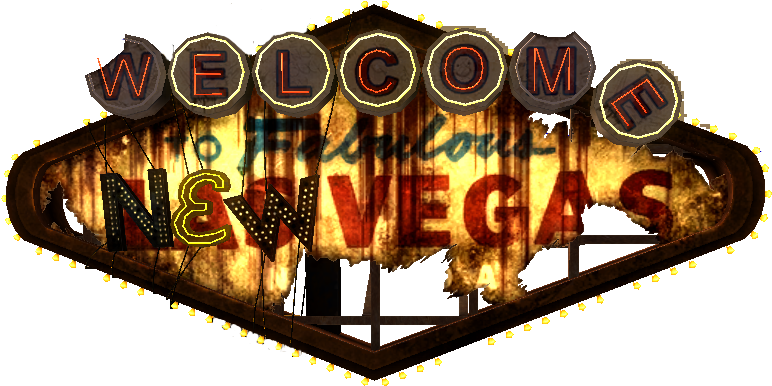
\includegraphics[scale=0.5]{logo_new_vegas.png}
\end{center}
\newpage
\tableofcontents
\newpage

\section{TODO}
\begin{itemize}
\item DAMAGES SUFFER DISREPAIR WHEN SKILL TEST FAIL, AND NEED TO BE REPAIRED
\item specify Ranger
\item adicionar vaults
\item adicionar mapas
\item Add traits? -- GHOULIFIED TRAIT
\item complete types of FEV strainss
\item review glowing one formula
\item remove casino descriptions from factions/strip subfactions
\item add base equipment for each class/race
\item review chars with 0 DT
\item global replace SPECIAL with S.P.E.C.I.A.L. 
\end{itemize}
\newpage

\section{INTRODUCTION}

\epigraph{\textit{I planned each charted course \\
Each careful step along the byway \\
And more, much, much more \\
I did it, I did it my way}}{\textit{``My Way'', Frank Sinatra}}

War. War never changes. The year is 2270. In the Mojave desert, the New California Republic spreads its influence. After a deal with Robert House, famed millionaire and owner of the most mysterious casino in New Vegas, the Lucky 38, the NCR starts settlements, fights off raiders, and seems to do a good job in bringing civilization to the desert for several years, even restarting Hoover Dam and increasing electricity supply to New Vegas. Then, the Legion arrived.

The year is 2277. Coming from Arizona, Caesar's Legion starts to move into the Mojave, starting by Fortification Hill, where they set their camp. Soon, under command of Legate Joshua Graham, the Legion moves to take over Hoover Dam. After an initial victory, the NCR lures the Graham to a trap, causing them to retreat. Humiliated, Caesar orders that Graham be coated in pitch, lit on fire and thrown into the Grand Canyon, to serve as an example. 

The year is 2281. The Mojave is largely under the influence of the NCR, but the Legion has started expanding. The town of Nipton, a hub of thievery and prostitution, is destroyed as a both a demonstration of power and as a way to send a moralizing message to New Vegas. The NCR begins to feel the weigth of the conflict, and people slowly begin to notice this. A new battle for Hoover Dam seems inevitable. 

From all over New Vegas, stories begin to crop up about a person who came back from the dead for revenge, in the small town of Goodspring. Very little is known about this person, except that they are called Courier Six. Along the way, this person helped a lot of people, restoring order and eliminating various threats to the citizens of the Mojave, accruing a reputation of being something of a Messiah. His actions tip the balance in favor of the NCR, and in the coming battle, his help is decisive in assuring the victory of the NCR.

The year is 2286, 5 years after final battle between NCR and Caesar's Legions. The Mojave is a changed place. The Great Khans stopped supplying chems to other factions, reconnecting to the Followers of the Apocalypse. The Brotherhood of Steel patrolled part of the desert, NCR handled the other. New Vegas poorest neighborhoods, Westside and Freeside, began to flourish. Although troubled by the taxes, NCR citizens experienced prosperity like never before. Caesar's Legion was no more.

That's where we begin.

\newpage

\section{CREATING YOURSELF}

\epigraph{\textit{Good authors, too, who once knew better words \\
Now only use four-letter words \\
writing prose. \\
Anything goes}}{\textit{Anything Goes - Cole Porter}}

The Mojave is not a safe place, that much must be clear to you. And how are you going to survive your voyages? Are you a brawler? A brainiac? A bamboozler? 

\subsection{You are S.P.E.C.I.A.L.}

You are S.P.E.C.I.A.L., as in, you are what your stats say you are. These 7 characteristics are the base of what you are, so the least you could do is know what they mean, right? And don't forget, these are scales of 1 to 10. You start with 1 in each one, and get 35 points to spread among them as makes sense to the \textit{you} you are trying to create. You may have more due to bonus, but not by assigning them from your initial point pool.

\begin{itemize}
\item \textbf{S}trength: do you want to carry a lot of weapons? Lift heavy rocks? Maybe your dream is to double-wield miniguns(you will likely not be able to do this, actually). All these, and more, are possibilities granted to you by investing in Strength. On the other hand, if you neglect it, you might not even be strong enough to properly wield your weapon

\item \textbf{P}erception: either by seeing what's beyond sight, identifying who's around by their footsteps, smelling like an old hound dog (and I mean detecting scent, please take a shower once in a while), don't forget to invest in Perception. After all, while surprise mauling by deathclaw may not be one of the leading causes of death on the Mojave, there is no reason to risk it, either

\item \textbf{E}ndurance: so you want to be tougher than the toughies? Strength is good, but endurance is better. You may hit like a brick, but it's worthless if you can't take a punch, or even fight properly. You are not a supermutant (or are you?), and even if you were, you should know what you're doing

\item \textbf{C}harisma: I was going to make a joke at your expense, but nah, you convinced me not to, you sweet talker you. Hey, maybe you deserve a discount on these stimpaks, eh? Just because you're so nice. You're lucky to be such a character, otherwise I might not even be talking to you

\item \textbf{I}ntelligence: so now you want to be smarter than the smarties? A regular wise guy, mister know-it-all, understand electronics, big words and figures out computers like they ain't no thing? Keep it up. You don't want to be a schmuck that can't figure his way out of his pants, dig?

\item \textbf{A}gility: you want to be fast, kid, if you want to escape deathclaws. Also, being able to climb the flimsiest ruins in the Mojave also helps a lot. As they say, if you can't be strong, at least be fast

\item \textbf{L}uck: keep in mind, you're in Vegas, so it won't hurt you to have a little luck. It may just save you in everything you do, except if what you're doing is winning too much on the cassinos. \textit{That} tends to not be very healthy
\end{itemize}

\subsection{Skills}

You are your stats, but you are also your skills. Do you barter? Blow stuff up? Beat people up? There are a lot of things you can do, to different levels of proeficiency. Keep in mind, skills go from 1 to 100. And, like S.P.E.C.I.A.L. stats, it can be increased by bonuses, over the 100 limit.

\begin{itemize}
\item \textbf{Barter (C):} be it caps, NCR money or other, less tangible currency, that's your game. Having a high barter will help you negotiate the best price for a mini-nuke, or explain to someone why leaving you alone is the most profitable solution. Provided that that someone is not a deathclaw

\item \textbf{Energy Weapons (P):} guns that go ``pew pew'' or that turn people into goo are your jam. Unlike their ``bang bang'' counterparts, they are more than point and fire, one needs to know how to regulate them properly, and keep all parts working properly

\item \textbf{Explosives (P):} you like it when things go boom, and you can make them go \textit{really} boom, while being safe from all the ill efects of all those booms

\item \textbf{Guns (A):} some people like lasers, some people like explosions, but you are the one who knows that a piece of metal through the head is enough to stop the toughest of foes. Provided, that is, that you are using the proper gun and ammo. And you are always using proper gun and ammo

\item \textbf{Lockpick (P):} you view keys are more of a philosophical choice, instead of a practical need. As long as you have a bobby pin, no lock wil ever deter you. Of course, you could use a gun, or explosives, but why would you let people know you're coming?

\item \textbf{Medicine (I):} maybe you like helping people, or maybe you just needed to patch yourself after the latest kerfuffle, but you know bones and cuts, and how to mend them, even and especially using chems

\item \textbf{Melee Weapons (S):} guns are for weaklings. Your pipe, knife, sword, spear, or even a rock will take you to victory, and you will never run out of ammo for them. Just don't get cocky, kid

\item \textbf{Repair (I):} you can fix your guns, you can fix your armor, you can fix your friend's machine. The only thing you can fix is the world around you. Or maybe you can?

\item \textbf{Science (I):} where other people see mysteries, you see mechanisms that you can manipulate. You know how to create, change and destroy chems, robots, computers

\item \textbf{Sneak (A):} wait, am I here alone explaining stuff to the air like a looney? Where are you? Hope you're not thinking of backstabb... 

\item \textbf{Speech (C):} unlike me, you can talk anyone into almost anything. Wait, what did you say? Oh sorry, I agree, you can talk \textit{anyone} into \textit{anything}

\item \textbf{Survival (E):} you are the person who makes medicine from plants, fire from two rocks and some twigs, and you are one of the few people who can actually turn radscorpion poison glands and a deathclaw egg in a meal fit for a king. All that in a cave that you made by yourself

\item \textbf{Unarmed (E):} you don't need any weapons, since you \textit{are} the weapon. You can say that with confidence, since no one that laughs at your corniness will regret it instantly

\end{itemize}

\subsection{Races}

Humans are the most common kind of people you will meet on your voyages, but not the only ones. Some people were mutated by radiation, better known as ``ghouls''. Also, some might be supermutants, in which case you should probably run away. Unless you yourself are a supermutant too.

\subsubsection{Average humans} 

You are the default race in New Vegas, found everywhere in most major cities and settlements. There is not anything notable about you, except your belief that Humans are better than ghouls, though you might tolerate them if you stand to gain something by their presence. Supermutants, on the other hand, are instinctively scary to you. Humans usually call ghouls ``zombies'', and there is no slur for supermutant. By default, humans don't get any alterations, but your specific background might change you. There are several variations of humans, according to how and where they were raised:
\begin{itemize}
\item \textbf{Vault Dwellers:} as the name implies, you are a human raised in a Vaults, descendant of people who went into Vaults when the bombs fell. Compared to the rest of the Mojave, you tend to have odd customs. A dead giveaway of your origins is the Pip Boy in your arm, though some wastelanders may have acquired Pip Boys from dead Vault Dwellers. Due to their more sheltered lives, Vault Dwellers in general get -1 Endurance, -1 Agility, +1 Perception and +2 Intelligence, though their specific vault background can change these or other stats, depending on the type of environment in which they grew up 
\item \textbf{Raider:} as a raider, you come from a culture that overvalues physical strength over intellectual prowess, a hedonistic life that does not accept feelings or dialogue. ``Might before right'' could be your motto. You get +1 Strenght and +2 Endurance, +20 Survival, +20 Guns, but their way of life costs them -1 Intelligence, -3 Charisma, -30 Barter, -20 Energy Weapons
\item \textbf{Strip Citizen:} your life on the Strip could not be considered easy, but it's easier than on other places. The casinos are your second home, and prostitutes are basically the only interesting girls you meet. This environment has taught you to solve your problems using either your gun, your mouth, or your dice. You get +2 Charisma, +1 Luck, +20 Speech, +10 Guns, but the cozy life leaves you with -1 Endurance and -1 Agility, and -20 Survival
\item \textbf{Freesider/Westsider:} unlike your counterparts from the Strip, you have had to learn how to handle themselves with little resources, getting +1 Strength, +3 Endurance, +20 Survival, +20 Melee, +30 Unarmed, +15 Repair. On the other hand, a hard knock life left you with -1 Strength, -1 Charisma, -3 Luck, and -20 Energy Weapons
\item \textbf{NCR Soldier:} life in the army has been good to you, yes siree. Discipline and training, and since your deployment on New Vegas, quite some hours piloting the slot machines and blackjack tables. You get +2 Endurance, +10 Explosives, +20 Guns, +5 Medicine, but it costs you in -1 Charisma, -10 in Energy Weapons. Also, serving in New Vegas means a lot of time spent in the casinos, which gives you +1 Luck
\item \textbf{Follower of the Apocalypse:} from birth, you have lived around a camp and helped take care of people in need. You have used chems as medicine, sutured open wounds, and did a lot of negotiation to get the resources you need. You get +2 Intelligence, +3 Charisma, +40 Medicine, +20 Science. However, a life dedicated to peace means you get -1 Strength, -10 Guns, -10 Explosives, -20 Energy Weapons, -30 Melee and -10 Unarmed
\item \textbf{Brotherhood of Steel:} as a Brother (or Sister), you were born with electricity coursing through your veins, being trained since a youngling into cutting-edge technology. Thus, you get +35 Energy Weapons, +20 Science, +10 Repairs and +2 to Intelligence. However, the isolationist and supremacist culture that surrounded you from birth took its toll, and you get -2 Charisma, -20 Speech, and since you were always taught to ignore them, -10 to Guns, -30 to Sneak and -20 to Survival. As a bonus, you are able to wear a Power Armor without training, provided your Intelligence is 4 or more
\item \textbf{Boomer:} forget about the Brotherhood of Steel, Boomers are the Mojave's premiere isolationist, chauvinist group. Descendants of the inhabitants of Vault 34, where all problems were solved at gunpoint, Boomers despise all people who they call ``savages'', with some of them dreaming of cleansing the Mojave with a bomber plane called ``Lady in the Lake''. Thus, you get +40 Explosives, +20 Guns, +20 Repair and +20 Science, but your antisocial tendencies will be obvious, with -4 Charisma, -30 Speech, and -20 Barter
\end{itemize}

\subsubsection{Ghouls}

You look like you were hit with a flamethrower, ghouls are best described by the words of the best DJ in post-apocalyptia, ThreeDog: ``Sure, they may look like hideous zombies from an old monster flick, but their hearts, their souls, their tears are all very much human. You see, children, Ghouls are simply humans who've been exposed to an ungodly amount of radiation and haven't had the good fortune to die.'' 

Though a lot of you remain essentially human, some ghouls become feral, losing all capacity to communicate or develop rational thinking, becoming little more than zombies from old movies. After some time being mistreated by them, you are likely to develop some amount of prejudice against the ``smoothskins''. Most of your ghoul friends have, at least.

On the physical side, part of the damage affected your vocal cords, meaning that you developed a raspy voice. But now you don't need to eat or drink, though you can do it if you can. You regenerate health in radioactive environments, although too much, too fast, may turn you into a Glowing One, and/or even turn you feral. You get +30 Survival, -1 to Endurance, -2 to Charisma, -1 to Agility, -20 to Barter, -20 to Speech
\begin{itemize}
\item \textbf{Feral Ghoul:} As a feral ghoul, you will lose all your social skills: Intelligence, Charisma, Barter and Speech become 1. You don't think, you don't have goals, and you live for the next meal, forever or until someone puts you out of your misery. You're done, kid. Hope it was nice while it lasted.
\item \textbf{Glowing One:} it's hard to reach this level of ghoulification without becoming feral, but it can happen. As a Glowing One, you can store radiation and release it as an energy burst (this action costs 2 Action Points) that restores your health, as well as the health of other ghouls in your vicinity. Sometimes, you might even resurrect a fallen ghoul this way. But you can kiss goodbye your chances of walking peacefully among humans, even though some might deal with you. The radiation makes you stronger than normal, and you get +2 Strength
\end{itemize}

\subsubsection{Supermutants} 

Large, green, strong, ugly and not very smart, let's hope you are not sensitive about this and, if you are, that nobody says that to your face. 

Supermutants are humans that were exposed to the Forced Evolution Virus (F.E.V.), and used to serve the Master, a megalomaniacal, superintelligent mutant (a different sort of mutant), and after his demise, became mostly directionless. Because supermutants are sterile, the usual way to increase their numbers is by capturing humans and exposing them to the F.E.V. (only humans, as ghouls are not affected). 

You get +3 Strength, +4 Endurance, +1 Perception, +2 Intelligence, +2 Agility and -5 to Charisma. Additionally, you get +5 to total strength, being able to reach 15, but you start with 25 S.P.E.C.I.A.L. points for your character, and +10 points to Damage Threshold, reflecting your superior durability. Due to their large hands, you will not be able to use most smaller weaponry, in either it's laser or gunpowder varieties, and forget about power armor, too, as they don't come in extra larger sizes. Supermutants normally ignore ghouls, though sometimes they might use them as slave labor. There are two possible variations to supermutants:

\begin{itemize}
\item \textbf{Nightkins:} you are the supermutant other supermutants aspire to be. As a nightkin, you are smarter, stronger and more resilient, but that makes them more arrogant. Thus, you get +5 to total strength, being able to reach 15, +4 Strength, +4 Endurance, +1 Perception, +2 Intelligence, +3 Agility and -6 to Charisma. Additionally, you get +6 to total strength, being able to reach 16, but you start with 25 S.P.E.C.I.A.L. points for your character, and +15 points to Damage Threshold, reflecting your superior durability.. In terms of appearanche, your overindulgence of Stealth Boys caused your skin to become more of a purple-ish skin tone, and you tend to be severely paranoid, going into full on schizophrenia in your worst moments
\item \textbf{Behemoths:} you much larger, stronger, dumber and more savage than regular supermutants. Though not completely feral, behemoths are not well fitted to do much besides smashing, though they can also be very caring with someone or something for which they have affection. You get +10 to total strength, being able to reach 20, +6 Strength, +6 Endurance, +3 Perception, +2 Agility, -6 Intelligence, -6 Charisma, +25 DT and your hands are too large to use most weapons, except for large blunt equipment and debris.
\end{itemize}

\subsection{Races summary}

It is important to note that there are more possibilities regarding backgrounds. What if, for instance, your character works with the Followers of the Apocalypse, but as a guard? This would likely negate the downsides regarding combat skills, but also the bonuses regarding Science, Charisma and Medicine. An exhaustive list would be impossible, but hopefully these backgrounds will inspire and guide you in crafting your character.

\begin{longtable}{|p{4cm}|p{5cm}|p{5cm}|}
\hline
\bfseries Race / Class & \bfseries Upside & \bfseries Downside \\
\hline
\endhead
\bfseries Human & None & None \\
Vault Dweller & +1 PE, +2 IN & -1 EN, -1 AG  \\
Raider & +1 ST, +2 EN, +20 Survival, +20 Guns & -1 IN, -3 CH, -30 Barter, -20 Energy Weapons \\
Strip Citizen & +2 CH, +1 LU, +20 Speech, +10 Guns & -1 EN, -1 AG, -20 Survival \\ 
Freesider / Westsider & +1 ST, +2 EN, +20 Survival & -1 CH, -2 LU \\
NCR Soldier & +2 EN, +1 LU, +10 Explosives, +20 Guns, +5 Medicine & -1 CH, -10 Energy Weapons \\
Follower of the Apocalypse & +2 IN, +3 CH, +40 Medicine, +20 Science & -1 ST, -10 Guns, -10 Explosives, -20 Energy Weapons, -30 Melee Weapons, -10 Unarmed \\
Brotherhood of Steel & +2 IN, +35 Energy Weapons, +20 Science, +10 Repairs & -2 CH, -20 Speech, -10 Guns, -30 Sneak, -20 Survival \\
Boomer & +40 Explosives, +20 Guns, +20 Repair, +20 Science & -4 CH, -30 Speech, -20 Barter \\
\bfseries Ghoul & +30 Survival, Health Regeneration under Radiation & -1 EN, -2 CH, -1 AG, -20 Barter, -20 Speech \\
Glowing One & +2 ST, +2 EN, +30 Survival, Health Regeneration under Radiation, Radiation Burst & -1 EN, -2 CH, -1 AG, -20 Barter, -20 Speech \\
\bfseries Supermutant & +3 ST, +3 EN, +1 PE, +2 IN, +2 AG, Radiation Immunity, +5 Total Strength, +10 DT & -5 CH, 25 starting S.P.E.C.I.A.L. points at the start, Can only use large weapons and can't use power armor \\
Nightkin & +4 ST, +1 PE, +4 EN, +2 IN, +3 AG, Radiation Immunity, +6 Total Strength, +15 DT & -6 CH 25 starting S.P.E.C.I.A.L. points at the start, Can only use large weapons and can't use power armor \\
Behemoth & +6 ST, +6 EN, Radiation Immunity, +10 Total Strength & -6 IN, -7 CH, 25 starting S.P.E.C.I.A.L. points at the start, Can only use special blunt weapons \\
\hline
\end{longtable}{\begin{center}Imagine all the possibilities. Then, imagine all the possibilities that are not here.\end{center}}

\subsection{Putting Everything Together}

So, that's half the battle, kid, because now you know. But let's put it together in an easy to-do list, to make things easy.

\begin{enumerate}
\item The easiest way to start a character is to start with a concept. Are you human? Ghoul? Supermutant? Think about those things, they will guide you in your next steps
\item Choose a race and apply buffs and debuffs
\item Set all your S.P.E.C.I.A.L. stats to 1, then allocate 35 points among them to start, unless you are a supermutant, who gets only 25 points
\item Select one trait from the list in Appendix \ref{app:traits}, then apply buffs and debuffs as appropriate. 
\item Calculate stats derived from the following formulas:
\begin{center}
Carry Weigth (CW) = $150 + (Strength * 10)$ \\
Health Points (HP) = $100 + (Endurance * 20) + ((Level - 1) * 5)$ \\
Sequence = $1d10 + Agility$ \\
Actions per turn = $ \lceil Agility / 2 \rceil $
\end{center}
\item Tag 3 skills, and no more than 3. 4 will not be chosen, neither will 2, except in the case that it's leading to 3. Forget about 5! Once 3 skills are tagged, the third being the last
\item For each Skill, use the formula below, then add 15 if it is a tagged skill
\begin{center}
Skill = $2 + (2 * S.P.E.C.I.A.L.) + \lceil Luck / 2 \rceil$
\end{center}

\end{enumerate}

\subsection{Level Up} 

Unlike war, you change. Your adventures around the Mojave will mold you, you'll become more adept at fighting, persuading, fixing things and people in more than one way. The simplest way is to use the following formula to calculate the amount of experience needed for the next level: 

\begin{center}
Next Level(n) = $25 * (3 * n + 2) * (n - 1)$, where $n$ is the current level
\end{center}

For instance, the experience needed to reach level 10 is:

\begin{center}
Next Level(10) = $25 * (3 * 10 + 2) * (10 - 1) = 25 * 32 * 9 = 7200$
\end{center}

When leveling up, the player gains an amount of skill points to distribute equal to the following formula:
    
\begin{center}
Skill points = $10 + \lceil Intelligence / 2 \rceil$
\end{center}

Finally, every three levels, you can choose a perk from Appendix \ref{app:perks}. Some perks can have more than one rank, that is, be chosen more than once.

However, this method is not exactly straightforward. Maybe it bothers you to get good at energy weapons when all you use is a minigun. A different approach is for the narrator to instead attribute points for successful use of skills, be it a constant value or dice based, and level up players as a result of one or more quests that the player undertake.

\begin{longtable}{|p{2.8cm}|p{1.8cm}|p{1.8cm}|}
\hline
\bfseries Difficulty & \bfseries Constant & \bfseries Dice \\
\hline
\endhead
Very Hard & 13 & 1d20 \\
Hard  & 9 & 1d12 \\
Average & 6 &  1d10 \\
Easy & 3 & 1d6 \\
Very Easy & 2 & 1d4 \\
\hline
\end{longtable}{\begin{center}Maybe you don't love dice, maybe you do. \\ We have options for all.\end{center}}

\subsubsection{An Example Character - Fink}

So, let's create a sample character. Say, this cat will be a Nightkin that is pacifist whenever able, although that's not very often in the wasteland. Being a former soldier for the Master, this kid has walked a long way to reach the Mojave, so he'll start at level 8. But first things first.

Let's start with a name. Let's go with ``Fink'', because someone called him that and he didn't know what the word meant, but liked the sound. Next, let's make like a waiter and focus on the S.P.E.C.I.A.L.S.. We start with 1 for each stat. Then let's check our bonuses, which are quite nice if I do say so myself: +4 ST, +1 PE, +4 EN, +2 IN, +3 AG, -6 CH. And since we already have the information handy, we can take note of our +15 DT. Then, we decide how to apply 25 SPECIAL points. 

Fink will be tough, silent type (very original, ain't I?). So, let's put +4 ST, +5 PE, +3 EN, leaving us with 12 points left. Let's put enough CH to leave us with something, so another 6 points there. Communication isn't his forte, but he can do the very basic, and we have 6 more points to apply. Seems fair to apply +4 IN, +3 AG. We'll neglect Luck, but if Fink was the lucky type, he probably would die without being exposed to the FEV, dig? 

Next, we'll choose a trait. For simplicity, let's choose Gifted, adding +1 to every SPECIAL stat, but getting -2 to every skill. Easy-peasy, lemon squeezy, so on to sort out our calculated stats: max CW is 150 + 10 * 10, which equals 250. Max HP is 100 + 9 * 20 + 7 * 5, adding to 295. Sequence is a 1d10 roll + Agility, giving us a nice 13. Finally, actions per turn is half agility, rounded up, which is 4.

Fink is coming out nicely, isn't he? So now let's move on to skills, and tag three of them. Fink is a former soldier that has had to survive without many friends for a long, long time, so it makes sense for him to have Guns, Survival and Unarmed. 

The last two steps will not be detailed for brevity, after all, they involve all 13 skill. But don't worry, I won't leave you hanging. Let's focus on two skills that would make sense for Fink: Speech and Unarmed. After all, not even Fink could avoid people forever. Speech is dependent upon Charisma, and Unarmed upon Endurance, so we'll do 3 + twice for each of those stats, for starters, which is 7 for Speech and 21 for Unarmed. Then, we need to apply our trait of Gifted, leaving the values as 5 for Speech and 19 for Unarmed. But these values are for level 1, and since then we've gained 7 more levels, accruing a total of 14 skill points per level times 7 levels, which is 98 skill points. Of course we would not apply all those points in just these two skills, so let's say we add 20 points for speech, so Fink can actually try to get things when force is not an option, and another 20 for Unarmed, for a total of 27 and 41. 

Lastly, every three levels we gain a perk, meaning we have two perks at level 8. Since he is a survivor, we'll give him Purifier and Hunter, so he can more adequately face strong creatures, dealing more damage. So, finally, we have Fink, ready for adventure. ONWARDS!

\subsection{External Influences}

Of course, you won't be altered only by your choices as a character. All along the Mojave, you'll find armor (see Appendix \ref{app:wearables}), weapons (see Appendix \ref{app:weapons}), chems (see Appendix \ref{app:chems}) and even the environment itself.

\subsubsection{Radiation}

Being close to radiation is enough to perceive that it's dangerous, but until the war, few humans imagined how dangerous it could be. The normal effect is \textbf{radiation sickness}, which causes progressively worse symptoms.

\begin{longtable}{|p{3.3cm}|p{3.1cm}|p{4.3cm}|}
\hline
\bfseries Rads & \bfseries Level & \bfseries Effect \\
\hline
\endhead
0-199 &	No Effect & - \\	
200-399 & Minor Radiation Poisoning & -1 END \\
400-599 & Advanced Radiation Poisoning & -2 END, -1 AGL \\
600-799 & Critical Radiation Poisoning & -3 END, -2 AGL, -1 STR \\
800-999 & Deadly Radiation Poisoning & -3 END, -2 AGL, -2 STR \\
1000+ & Fatal Radiation Poisoning & DEATH (HP: -10,000) \\
\hline
\end{longtable}{\begin{center}Watch out for those rads. They hurt. A LOT.\end{center}}

Some lucky ones, or maybe unlucky ones, through their exposition, suffer physical mutations, a process that is called \textbf{ghoulification}. They begin lose all hair, and suffer terrible burns on all skin, which becomes rough, at least what little skin remains attached to the body. Those afflicted with this condition resemble zombies from bad old horror flicks. The factors that cause ghoulification are not known, and to the unknowing eye, appear to be random.

Every time a player advances a level of radiation sickness, they get another level of ghoulification. Roll 1d10, and if the value is lower or equal to the current level of ghoulification, they suffer the symptoms all the symptons up to their level, according to the table below. For instance, if a player fails a ghoulification check at level 3, their character starts to experience partial hair loss, minor burns \textit{and} occasional voice raspyness. 

\begin{longtable}{|p{2.8cm}|p{10cm}|}
\hline
\bfseries Ghoulification Stage & \bfseries Effect\\
\hline
\endhead
1 & Voice occasionally becomes more raspy, like a sore throat \\
2 & Minor burnt-like lesions on the skin \\
3 & Voice becomes permanently raspy \\
4 & Loss of chunks of hair \\
5 & Skin loss with no skin regeneration \\
6 & Flesh assume the burned appearance \\
7 & The player is now fully feral \\
\hline
\end{longtable}{\begin{center}You always knew ghoulification was unpleasant, but did you expect something like this?\end{center}}

If the player either a) is a ghoul already and takes radiation enough to move over three levels at once (that is, over 600 rads in a short period of time\footnote{One turn, or to the Narrator's discretion}) or b) takes over 800 and the player already has at least one level of ghoulification, they risk becoming a Glowing One. To determine if the player became a Glowing One, roll 1d10: the transformation occurs if the result is greater than the current ghoulification stage plus 2.

So, essentially, there are two steps to moving a player's ghoulification level up:
\begin{enumerate}
\item Check the next stage in the player's ghoulification meter
\item Ghoulification = True if 1d10 $>$ player ghoulification stage + 2, otherwise False
\end{enumerate}

\subsubsection{Exposure to the F.E.V. TODO}

This is not your everyday occurrence, but it may happen. Supermutants will throw their prisioners, or perhaps it would be more precise to call them ``future siblings'', on large tanks filled with a strange liquid infused with the Forced Evolution Virus (F.E.V.). After some time, the former human emerges as an enormous green brute, stronger, more agile, more perceptive, and more.

However, things are not that simple.

For starters, F.E.V. subjects should have little radiation damage (i.e. low ghoulification level) to avoid complications in the mutations that the virus causes, otherwise the radiation will cause damage to the mutation process, and these changes are always negative. Another important detail is that there are multiple strains of the F.E.V., though only some of them affect humans. 

The \textbf{F.E.V.-II} is the strain that is used to create supermutants. It is derived from the F.E.V.-I, a pre-war strain that was intended to be used as a military weapon. This virus is immune to radiation, which is part of the process to create 

chance to cause increase of increase intellect (1d10/ 2 for increase, 3 for reducing, 5 for staying the same)



EEP Strain, from FO3


\subsubsection{Power Armor}

Power armor is, as you might have deduced from it's name, \textit{powerful}. Some could say that it will make you feel like some sort of invincible robotic man made of iron. Wearing it, you no longer need to worry about small guns, minor explosions (provided you can get up fast), but sorry, Deathclaws will only see you as really tough canned food. But rejoice, as falling long falls no longer harms you, though it does cause a small tremor near your landing spot that will hurt and stun people around you, which is a good advantage in combat, so keep this in mind. Also, hurting people makes them like you less, so keep this in mind as well.

\subsubsection{Chems}

Heeyy, maan, chems are fuuun, riiight? Yes, they are, and they will make you better than you are, for a time... and for a price. The price you pay for chem usage is addiction. Addiction is cumulative. Every time you use a chem, it adds 10\% to the cumulative percentage to get addicted to that substance. Then, to find out if you're addicted, roll 1d100 against the probability to get addicted to the used substance. If the value is lower than current addiction probability, congratulations, now you feel like shit every time you're not under the influence, isn't that nice? Addiction probabilities reduce 10\% for each night of good rest, and addiction itself can be cured by going cold turkey for one in game week, or by going to your local phisician. For a detailed list of effects, once again, check Appendix \ref{app:chems}. 

\newpage

\section{THE WORLD}

Well, now you know a bit more about individuals of this world, or at least how to be one. Next step is to learn about the places in this world, and its tribes. We'll start with the latter.

\subsection{Factions}

Few things survived the bombs. 

\begin{itemize}
\item \textbf{New California Republic (NCR):} The NCR is an ever-expanding that started in the town of Shady Sands, in New California. Their political structure is very similar to the old USA, with a president, congress, corruption and inefficiency. Although very successful in their expansionist campaign, the Mojave seems to be where they are spread thinnest, and people are starting to notice. After the signing the The Ranger Unification Treaty, which unified their military with the Desert Rangers, a paramilitary group from Nevada that also fought against Caesar's Legion
\begin{itemize}
\item \textbf{Rangers:} 
\end{itemize}

\item \textbf{The Strip:} The Strip is the most luxurious area in New Vegas. The only entrance is through Freeside, by having 2000 caps (no need to pay, just need to have the money to spend), a passaport, or by being a member in good standing of the NCR, as NCR personnel frequent the Strip during downtime. The Strip has four casinos, each with their own group:

\begin{itemize}
\item \textbf{The Tops (Chairmen):} Home of the best showhouse in New Vegas, the Aces Theater, The Tops is a luxurious hotel-casino. It is commanded by the Chairmen. The Chairmen are a faction self-styled after the old Vegas, and the hippest cats around, dig? As in ``no finks allowed''. Civilized by Mr. House, they used to be a tribe known as the Mojave Boot-Riders, but now are the former most important faction in New Vegas, position they lost when their former leader, Benny, got what was coming to him for shooting Courier Six in the head. Currently, their main goal is to get back to the top, without crossing the Securitrons

\item \textbf{Gomorrah (Omertas):} Home of the Brimstone, the best strip club in New Vegas. Managed by the Omertas, a faction that follows the best traditions of the \textit{cosa nostra}. Though they lack the acce nt and the lingo, they very much love power and control. Five years ago, their leaders were killed by the current leader, Cachino, and the Courier Six. This happened after Courier Six uncovered a plot for a hostile takeover of the Strip by the former leadership, aided by Caesar's Legion. Since then, the Omertas have been very quiet. Maybe too quiet...

\item \textbf{Ultra-Luxe (White Glove Society):} Home to the Gourmand, the best and most exclusive restaurant in New Vegas, and the only place where one can find the Strange Meat Pie. Previously ran by a mysterious group that who wore gloves, fancy porcelain masks and haute couture clothing, the truth was that most of their members were cannibals. Courier Six and Yes Man cleaned the house up, and now there is zero human meat consumption on the premises, or so it seems. Very little is known about its current staff

\item \textbf{Lucky 38 (Securitrons):} For many years, nobody entered the Lucky 38. That is, until 2281, when Courier Six was invited by the very owner, Mr. House. However, the hospitality was paid with a bullet from Maria, Benny's 9mm. Soon after, Yes Man replaced House in controlling all Securitrons, who became the staff for the Lucky 38, the most luxurious hotel-casino in the strip. Nowadays, the panoramic cocktail lounge has the best drinks, and a full reservations lists for weeks, and all is managed by Yes Man (who acts more like a ``Maybe Man'', after being reprogrammed with more autonomy), and is owned by Courier Six. Securitrons also serve as the main security force in the Strip, Freeside and Westside
\end{itemize} 

\item \textbf{Freeside:} right next to the Strip is Freeside, New Vegas' premiere slum. One of the best places to get robbed by random thugs armed with metal pipes and planks. If getting mugged is not your thing, you can find some of everything (or so they say) at Mick and Ralhp's, blow your money on the Atomic Wrangler Casino, or get in contact with the Followers of the Apocalypse at the Old Mormon Fort

\begin{itemize}
\item \textbf{The Kings:} the only gang that remain in Freeside, since Courier Six nixed the Van Graffs, the Kings are a group of gangbangers inspired in an old religious figure, known only as The King, which is also how their leader is called. A Kings member is easily identified by his black cowlick, peculiar speech, leather jacket, white t-shirt and jeans. Along with the Securitrons, they keep Freeside safe, holding considerable influence on local events
\end{itemize}

\item \textbf{Raiders:} Raiders are gangs of marauders that roam the Mojave wasteland, attacking those that seem more vulnerable. They tend to use melee weapons or low-grade guns

\begin{itemize}
\item \textbf{Fiends:} maybe some of the worst the Mojave has to offer, the Fiends are junkies that think about little more than raiding and using chems, and who respect only brute force. They used to buy mostly from the Khans, but are currently becoming more and more desperate looking for a steady flow, since the Khans have mostly turned inwards. They use regular clothes, raider armors and helmets made from the skulls of animals

\item \textbf{Jackals:} strong competitors for the title of worst the Mojave has to offer, the Jackals are not addicted to chems, but they are almost entirely cannibalistic. They are originated from Vault 15, in New California, though rarely they have the characteristic Pip Boy. Their group leaders tend to wear Metal Armor, distinguishing themselves in a crowd

\item \textbf{Scorpions:} a minor gang, they are a leaderless band of raiders that mostly live from attacks attacking caravans, and usually getting their asses handed to them by Fiends. They almost always wear mercenary cruises

\item \textbf{Vipers:} a rarer sight than the other gangs mentioned, the Vipers used to be more shamanistic. Also originated from Vault 15, the Vipers were nearly exterminated by the Khans, and today exist only in minor pockets throught the Mojave, dealing drugs and dreaming of better days
\end{itemize}

\item \textbf{Followers of the Apocalypse:} unlike most other factions, the Followers of the Apocalypse do not impose themselves by strength, but instead they are a force for helping all those in need, although they usually make a healthy exception for raiders. Composed mostly by intellectuals, the Followers have, among their ranks, physicians, chemists, and engineers. Every once in a while, some more combat-capable people end up attached to them, and are begrudgingly accepted as a necessary part of life in the Mojave

\item \textbf{Great Khans:} although they are a raider tribe, it would be foolish to mix them with the likes of the Fiends or the Jackals. The Great Khans base their entire culture on what literature they could find about the Mongolian empire, with a great emphasis on warrior's honor. The Khans make a living mostly by supplying drugs for most of the Mojave. Currently, the tribe is focused inwards, working alongside the Followers of the Apocalypse to restore themselves to their former glory. However, the Massacre of Bitter Springs is not forgiven, nor forgotten

\item \textbf{Brotherhood of Steel:} the Brotherhood of Steel is a military-religious organization that see themselves as annointed with the task of gathering technology, regulating its use and keeping it from the rest of the world. Once isolationists, the New Vegas chapter of the organization opened its doors to work with the NCR on the Battle of Hoover Dam, though they still refuse to share their tech, and since then they help patrol the Mojave, staying mostly near their secret base around Sloan, Novac, Primm and Goodpsprings 

\item \textbf{Caesar's Legion Remnants:} previously a large and arrogant army, the Battle of Hoover Dam left Caesar's Legion a shadow of their former selves. Most of the survivors from the Battle of Hoover Dam were imprisioned by the NCR on NCR Correctional Facility. Many deserters have retreated to Cottonwood Cove, where they live in total isolation

\item \textbf{Boomers:} Boomers are the former occupants of Vault 34, a Vault where divergences were solved with weapons. After a riot where most of the vault was destroyed, Boomers moved to Nellis Air Base, where they lived in isolation from those they called ``savages'' until Courier Six showed up at their doorstep and began a reintegration process. Currently, Boomers still view most of the ``savages'' with disdain, they have a good relationship with the NCR military, with some Boomers taking positions in the army, and a training program where select officers spend some time living among Boomers

\item \textbf{Black Mountain Clan:} once known as ``State of Utobitha'', after its ruler, Tabitha, the Black Mountain is a heavily irradiated area the once housed a satellite array. After Tabitha resumed her voyages, a supermutant named Marcus took over leadership over his peers that didn't want to go to Jacobstown. Marcus str
ives to estabilish diplomatic relations with humans, although that is not always possible

\item \textbf{Jacobstown:} a little town estabilished on what once was a luxury mountainside hotel, Jacobstown is where supermutants go to live in peace, and especially where nightkins go to receive help from the problems that the abuse of Stealth Boys cause. They are self-sufficient and segregationists, although that is not violently enforced, but both humans and supermutants seem happy to remain that way

\item \textbf{Powder Gangers:} a group of prisioners that took over NCR Correctional Facility, the Powder Gangers are easily identified by their clothes, typical dressing for the prision staff, and their predilection for explosive weapons, especially dynamite sticks and grenade launchers, and also low-grade guns like 9mm pistols and varmint rifles. Most of them were dizimated by the coordinated action of the NCR with Courier Six (mostly it was Courier Six)

\item \textbf{Westside:} in the old days, Westside was a slum that made Freeside look and feel like The Tops. However, its residents were resourceful and self-sufficient, vastly improving conditions on the neighborhood, especially since Courier Six solved the Fiends problems that plagued them

\begin{itemize}
\item \textbf{Westide Militia:} citizens dedicated to protecting Westside, who have courage and stubborness that compensate for their lack of training. Nowadays, they are financed by The Thorn, who supply them with Sniper Rifles and 10mm pistols

\item \textbf{The Thorn:} once an underground arena, where wastelanders put their mettle to the test by engaging in 1 on 1 combat against the wastelands many beasts, they have expanded their business to include an underground casino, which quickly is allowing Westside to become a veritable power on the Mojave
\end{itemize} 

\item \textbf{Searchlight Ghouls:} once members of the Bright Brotherhood, a cult of ghouls that dreamed of flying rockets to undertake ``The Great Journey''. After surviving the crash landing, they walked the Mojave for a long time, until they reached the town of Searchlight. The radiation from the Searchlight Disaster made the town a comfortable environment for them, also being intolerable for non-ghouls, which allowed them to live in relative peace. Perhaps, a little too much peace, even...

\item \textbf{Cities:} for the purposes of reputation, each city counts as its own individual faction.

\end{itemize}

\subsection{Main Cities and Settlements TODO}

\begin{itemize}
\item \textbf{The Strip:} The Strip is the heart of New Vegas, though to access this heart, one needs caps. A lot of caps. To be left through by the three Securitrons that guide its only access, a person must have over 2000 caps in their possession (it's not an entry fee, just a verification of wealth) or a passport. Having gone through the door, one is greeted by a long street where only the more affluent, and NCR soldiers, circulate, under the watchful eyes of Protectrons. Besides all the best casinos in Vegas, it's where are located the NCR embassy, Vault 21, and the train that runs between The Strip and Fort McCarran. 
\begin{itemize}
\item \textbf{The Casinos:} All four casinos share much in common: blackjack tables, slots, luxury rooms, and a proihibiton of carrying arms inside (although sneaky patrons tend to overlook this rule). The main differences are \textit{décor} and main attraction. 
\begin{itemize}
\item \textbf{Lucky 38:} it is the most luxurious casino, with a famous panoramic cocktail lounge that allows its patrons to see the most of the Mojave. It's whole staff is composed by reprogrammed Securitrons, which makes it the safest casino of all. It's managed by the Yes Man, on behalf of its owner, The Courier.
\item \textbf{Gomorrah:} managed by the Omertas, Gomorrah puts the ``sin'' back in ``casinos''. It's main attraction is the strip club, the Brimstone. After the failed alliance with Caesar's Legion, they saw a notable decrease in attendance, since practically all NCR soldiers started boycotting the establishment.
\item \textbf{The Ultra-Luxe:} though they claim to be the most luxurious experience available in the region, nowadays they are a distant second. Even with all the efforts of the new White Glove Society, their services can't match the speed and quality of the Securitrons from Lucky 38, though the restaurant The Gourmand is still the most notable on the region, especially since all rumours about it serving human meat have been quelled.
\item \textbf{The Tops:} former best casino of Vegas, it is managed by the Chairmen, a former tribe styled after the cool casino mafia from the past, with nice suits but also a good right hook. The Tops has the best showhouse around, with such cool acts as the musician Lonesome Drifter and the ghoul comedian Hadrian.
\end{itemize}
\end{itemize}

\item \textbf{Westside:}

\item \textbf{Freeside:} the poor neighborhood that surrounds the Strip, Freeside has a lot of rundown buildings used as shelter by it's inhabitants. A single pipe supplies water for everyone, and a member of the Kings is tasked with keeping distribution reasonable. Home to Mick and Ralph's, a shop where you can find almost anything, for the right price. Finally, it was also where the energy gun store Van Graff was located, before the Courier killed all of them for crimes that were never fully judged.
\begin{itemize}
\item \textbf{Atomic Wrangler:} the best casino outside the strip, the Atomic Wrangler is a rundown joint that has musicians, blackjack, hookers. They sell high quality drugs, though, due to their impressive labs, created and supplied by the Followers of the Apocalypse.
\item \textbf{The King's:} an old religious temple, The King's School of Impersonation still holds relics from the deity of its time, a man known only as the King. This ancient religion inspires the gang that currently occupies the building, the Kings, who follow in the King's image and mannerisms.
\end{itemize}

\item \textbf{Old Mormon Fort:} an old fortress in the middle of Freeside occupied by the Followers of the Apocalypse, the Old Mormon Fort has two towers that serve as quarters for the Followers. Inside its yard are laid several tents, as well as the foundations of a new hospital being built from the money the Followers made by keeping the distillery in the Atomic Wrangler in working condition.

\item \textbf{Goodsprings:} a western small town, it has a few still inhabitable houses, a general store, a Doctor's house and a saloon. It is also the famous as the place where the Courier was brought back from the dead. This has caused the town to receive many visitors, among them sickly people looking to be saved just like the Courier was.

\item \textbf{Primm:} 

\item \textbf{Novac:}

\item \textbf{Hidden Valley:}

\item \textbf{Nipton:}

\item \textbf{Cottonwood Cove:}

\item \textbf{NCR Correctional Facility:}

\item \textbf{Fort McCarran:}

\item \textbf{Nellis Air Base:}

\item \textbf{Jacobstown:}

\item \textbf{New Vegas Sewers:}

\item \textbf{The One:} Rumor has it that somewhere out in the Mojave lies one of the atomic bombs from the great war, undetonated. Those who have seen it, or who know about it, call it ``The One''.

\item \textbf{Bitter Springs:}

\item \textbf{Red Rock Canyon:}

\item \textbf{NCR Bases:}

\item \textbf{Searchlight:}
\end{itemize}

\section{A Little Bit of History TODO}

\begin{itemize}
\item \textbf{First Battle of the Hoover Dam}

\item \textbf{Second Battle of Hoover Dam}

\item \textbf{Pacification of the Three Tribes}: What each tribe waas and what they became

\item \textbf{Massacre of Bitter Spring}

\item \textbf{Operation: Sunburst}

\item \textbf{Massacre of Nipton}

\item \textbf{Searchlight Disaster}

\item \textbf{The Double Bombing:} When the Courier bombed NCR and Legion -- no one knows who it was. Legend says it was the Courier, but they denied, and there were no witnesses
\end{itemize}

\newpage

\section{Interactions HEAVY TODO}

\epigraph{\textit{When an irresistible force such as you \\
Meets an old immovable object like me \\
You can bet just as sure as you live \\
Somethin's gotta give}}{\textit{Something's Gotta Give - Bing Crosby}}

\subsection{Combat}

    Combat Basics
        Combat happens in a turn structure, where each character has a number of actions expressed by
            * $Actions = \lceil Agility / 2 \rceil$

        Each action can be one of the following:
            * Use an item
            * Perform an attack
            * Change or reload weapons
            * Prepare to block an attack
            * Run, hide or similar action
        A player can spend an additional action to perform an Aimed Shot.

        $Hit = 1d100 < Skill for the weapon type$

        $Damage for a weapon = Weapon's dice damage * (50 + Skill) / 100¹ - Target's DT$
        ¹ For ease, round it up
        
        $Melee Damage = Weapon's dice damage + \lceil Strength / 2 \rceil - Target's DT$

        $Unarmed Damage = \lceil Unarmed skill / 20 + 0.5 \rceil - Target's DT$

        Knockdown - If a melee attack causes damage over 30\% of the targets health, defending player must run a saving throw of 1d10 against their endurance

        Crippling damage - [HOW CRIPPLE WORKS]

        Sneaking damage - If the player is sneaking and undetected, multiply the final damage of the attack by 1d6 + 1

        Aimed Shot - For the cost of an extra action, the player can aim a shot to a specific part of the target's body. Precision calculation table?
        
        Spread - Multiplication of dice values is done to simulate the spread of automatic weapons like machine guns and miniguns
        
\subsection{Gambling}

\subsection{Disguises}

Some wearables are characteristic of a certain faction. By putting them on, people might not know that you're the person that they hate (or love). Just remember to avoid characters that would recognize you, and steer clear of factions that hold animosity towards the one you're impersonating. Remember: people rarely believe sentences like ``I swear I'm not a raider, I'm just wearing raider armor''.


\subsection{Reputations} 

The reputation is the summary of the relationship between a player and a faction. Do things that please a faction, and you'll be accepted, maybe even idolized. More realistically, sometimes you'll have to choose between two factions, and the one you don't choose will certainly not be happy with you. The people will remember you, so make those memories a good one.

\begin{longtable}{|p{2.3cm}|p{2.3cm}|p{2.3cm}|p{2.3cm}|p{2.3cm}|}
\hline
\textbf{±}  & \textbf{Level 1} & \textbf{Level 2} & \textbf{Level 3} & \textbf{Level 4} \\
\hline
\endhead
\textbf{Level 1} & Neutral & Accepted & Liked & Idolized \\
\hline
\textbf{Level 2} & Shunned & Mixed & Smiling Troublemaker & Good-Natured Rascal \\
\hline
\textbf{Level 3} & Hated & Sneering Punk & Unpredictable & Dark Hero \\
\hline
\textbf{Level 4} & Vilified & Merciful Thug & Soft-Hearted Devil & Wild Child \\
\hline
\end{longtable}{These are the ways you may be known throught the Mojave...}

\begin{longtable}{|p{3cm}|p{9cm}|}
\hline
\bfseries Reputation & \bfseries Meaning \\
\hline
Neutral & People don ' t know enough about you to form an opinion. \\
Accepted & Folks have come to accept you for your helpful nature. \\
Liked & Enough news of your good works has been passed around that people like you. \\
Idolized & Renowned for your extensive support and goodwill, you are idolized by the community. \\
Shunned & You ' ve left a poor impression on the community and may be shunned as a result. \\
Mixed & A little bit good mixed with a little bit bad, people haven ' t figured you out yet. \\
Smiling Troublemaker & People know you ' re good at heart even though you ' re occasionally a troublemaker. \\
Good-Natured Rascal & Your reputation as a good-natured friend of the community manages to outshine your dark side. \\
Hated & Now that folks know you ' re bad, most people outright hate you. \\
Sneering Punk & Even though you ' ve done some good for the community, people still think you ' re a punk. \\
Unpredictable & No one ' s sure what to make of your unpredictable nature, but you ' ve left a strong impression. \\
Dark Hero & Folks still think you ' re some kind of hero, but you sure can be nasty sometimes. \\
Vilified & For your overwhelmingly monstrous behavior, you have become vilified by the community. \\
Merciful Thug & Despite your reputation as a thug, you are known to occasionally show a charitable side. \\
Soft-Hearted Devil & Most people say you ' re the devil himself, but most admit you ' ve also done a world of good. \\
Wild Child & Your wild, seemingly capricious behavior leaves people scratching their heads in confusion and avoiding close contact. \\
\hline
\end{longtable}{... and this is what they mean, in practice}

\subsection{Sneak}

If no one is looking for the player character, they run a test against sneak.
If you're in an (N)PC line of sight, you need a critical success to be able to remain hidden. Stealth Boys guarantee success in this, except in the case of critical failure


\newpage

\appendix
\addtolength{\oddsidemargin}{-0.4in}
\addtolength{\evensidemargin}{-0.4in}
\addtolength{\textwidth}{0.8in}
\section{TABLES}

\subsection{TRAITS}
\begin{longtable}{|p{3.4cm}|p{6.5cm}|p{6.5cm}|}
\hline
\bfseries Name & \bfseries Upside & \bfseries Downside \\
\hline
\endhead

Bruiser & +2 ST & -2 AG \\
Chem Reliant & Addiction recovery is now 30\% PE night of good rest & Twice the chance to get addicted \\
Chem Resistant & Half the chance to get addicted & Chems last half as long \\
Claustrofobia & When outside you gain +1 to all SPECIAL stats & W hen indoors, you suffer -1 to all SPECIAL stats \\
Fast Shot & Get two additional action points that can be used exclusively to shoot & Cannot use Aimed Shot for any attack. \\
Feral Kid & +2 ST, +2 EN, +20 Unarmed, + 20 Melee Weapons, +20 Survival & -2 CH, -2 Intelligence, -20 Guns, - 40 Energy Weapons, - 30 Repair \\
Finesse & For every roll that is not a positive critical, you can repeat the roll twice and select the better result & - 10 overall damage \\
Gifted & +1 to all SPECIAL stats & - 2 to all skills, 3 less skill points at level up \\
Good Natured & +15\% to First Aid, Doctor, Speech, and Barter & -10\% to Small Guns, Big Guns, Energy Weapons, Throwing, Melee Weapons, and Unarmed \\
Heavy Handed & + 6 Melee Damage, +4 Unarmed damage & - 20 Repair, -30 Medicine \\
Jinxed & All criticals are negative for people around you & All your criticals are negative too \\
Kamikaze & +5 Sequence & Armor Class starts at 0\% \\
NCR Background & Find NCR caches and get extra background info & Bad reputation with other factions (WHICH?) \\
One Hander & +20\% chance to hit with one-handed weapons & -40\% chance to hit with two-handed weapons \\
Skilled & + 5 to all skills & Get a perk every four levels \\
Small Frame & +1 AG & Carry Weight = 25 + (15 x your ST) \\
Walking Ghoul & Higher chance to become ghoulified and Glowing & \\
\hline
\end{longtable}

\label{app:traits}

\subsection{PERKS}
\begin{longtable}{|p{3.3cm}|p{3.1cm}|p{1.2cm}|p{8.4cm}|}
\hline
\bfseries Name & \bfseries Other reqs & \bfseries Ranks & \bfseries Description \\
\hline
\endhead

Action Boy / Action Girl & AG 6 & 2 & Rank 1: +1 AG Rank 2: +1 AG +1 ST \\
Adamantium Skeleton & & 1 & Only cripple limbs on critical \\
Animal Friend & CH 6, Survival 45 & 2 & Rank 1: hostile animals become friendly Rank 2: they come to your aid against enemies except against other animals \\
Better Criticals & PE 6, LK 6 & 1 & + 3d6 damage with critical hits \\
Black Widow / Lady Killer & & 1 & + 2d6 damage to the opposite sex and positive reaction on all except negative critical \\
Cannibal & & 1 & Y ou can eat a human corpse to regain hit points, but lose reputation if witnessed \\
Center of Mass & Guns 70 & 1 & In Aimed Shots, you do an additional +1d 20 damage when targeting the torso \\
Chem Resistant & Medicine 60 & 1 & Half as likely to get addicted \\
Chemist & Medicine 60 & 1 & Chems last twice as long, stimpacks heal an additional 100 HP \\
Cherchez La Femme / Confirmed Bachelor & & 1 & + 2d6 damage to the same sex and positive reaction on all except negative critical \\
Commando & & 1 & +25\% accuracy in Aimed Shots with two-handed weapons \\
Comprehension & IN 4 & 1 & You gain one additional skill point for reading books and double the skill points for reading magazines \\
Computer Whiz & IN 7, Science 70 & 1 & Can hack any earthly computer \\
Cowboy & Guns 45, Melee 45 & 1 & + 2d6 damage done by dynamite, hatchets, knives, revolvers, and lever-action guns \\
Demolition Expert & Explosives 50 & 3 & + 2d6 damage with explosives \\
Educated & IN 4 & 1 & You gain two more skill points every time you advance in level \\
Entomologist & IN 4, Survival 45 & 1 & You do an additional 3d6 damage every time you attack a mutated insect \\
Fast Metabolism & & 1 & + 4d6 Hit Points restored with stimpaks \\
Ghastly Scavenger & Cannibal perk & 1 & You can eat a super mutant or ghoul corpse to regain hit points, but will lose reputation if witnessed \\
Gunslinger & & 1 & +25\% accuracy in Aimed Shots with one-handed weapons \\
Hit the Deck & Explosives 70 & 1 & +25 DT against explosives \\
Hunter & Survival 30 & 1 & In combat, you do 4d6 more critical damage against animals and mutated animals \\
Intense Training & & 10 & You can put a single point into any of your SPECIAL attributes \\
Laser Commander & Energy Weapons 90 & 1 & You do an extra 2d6 damage and have a 20\% extra chance to critically hit with any laser weapon \\
Lead Belly & EN 5 & 1 & -50\% Rads taken from food and water sources \\
Life Giver & EN 6 & 1 & + 60 hit points \\
Light Step & PE 6, AG 6 & 1 & Floor traps or mines will not be set off \\
Meltdown & Energy Weapons 90 & 1 & Foes killed by your Energy Weapons emit a corona of harmful energy, causing 1d6 of damage to characters nearby \\
Miss Fortune & LK 6 & 1 & Before using Aimed Shot, roll a Luck check. On success, Miss Fortune will appear and kill the target, then disappear. There is no way to interact with Miss Fortune \\
Mister Sandman & Sneak 60 & 1 & Can instantly kill a sleeping non-player character and earn bonus XP when doing so \\
Mysterious Stranger & LK 6 & 1 & Before using Aimed Shot, roll a Luck check. On success, the Stranger will appear and kill the target, then disappear. There is no way to interact with the Stranger \\
Nerd Rage! & IN 5, Science 50 & 1 & +15 DT and ST increased to 10 whenever health is 20\% or lower \\
Ninja & Melee Weapons 80, Sneak 80 & 1 & +30\% critical damage chance with unarmed attacks, melee or silenced weapons, +25\% damage, rounded up, with melee/unarmed sneak attack criticals \\
Pack Rat & IN 5, Barter 70 & 1 & Items with a weight of two pounds or less now weigh nothing \\
Paralyzing Palm & Unarmed 70 & 1 & Can paralyze an enemy for 2 turns with an Unarmed Aimed Shot (roll an Unarmed check) \\
Piercing Strike & Unarmed 70 & 1 & All your unarmed and melee attacks negate 15 points of DT \\
Plasma Spaz & Energy Weapons 70 & 1 & You get two Action Points exclusively for use with plasma weapons each turn \\
Power Armor Training$^1$ & IN 6, Science 50 or IN 8 and Science 75 & 1 & You can understand how a Power Armor works and use it efficiently \\
Purifier & - & 1 & You do 3d20 extra damage with melee and unarmed weapons against centaurs, night stalkers, spore plants, spore carriers, deathclaws and super mutants \\
Pyromaniac & Explosives 60 & 1 & +4d6 damage with fire-based weapons \\
Quick Draw & AG 5 & 1 & +2 to Sequence \\
Rad Child & Survival 70 & 1 & Instead of dying of radiation poisoning, advance one ghoulification stage and drop your rads to 400 \\
Rad Resistance & EN 5, Survival 40 & 1 & +25\% Rads resistance permanently \\
Rapid Reload & AG 5, Guns 30 & 1 & Don’t need to take an action to reload \\
Robotics Expert & Science 50 & 1 & +3d6 damage to robots; can shut down robots by sneaking up on them and deactivating \\
Shotgun Surgeon & Guns 45 & 1 & When using shotguns, regardless of ammunition used, you ignore an additional 10 points of a target's Damage Threshold \\
Silent Running & AG 6, Sneak 50 & 1 & You can run while sneaking \\
Slayer & ST 7, AG 7, Unarmed 90 & 1 & Get one extra action when using melee or unarmed attacks \\
Sniper & PE 6, AG 6 & 1 & 25\% more likely to hit the target's head with Aimed Shots \\
Stonewall & ST 6, EN 6 & 1 & +5 DT against melee and unarmed attacks and cannot be knocked down during combat \\
Strong Back & ST 5, EN 5 & 1 & +50 Carry Weight \\
Tag! & & 1 & Fourth ``tag'' skill: +15 points to that skill \\
Terrifying Presence & Speech 70 & 1 & +2d6 when trying to intimidate a character through dialogue  \\
The Professional & Sneak 70 & 1 & Your sneak attack criticals with revolvers, pistols, and submachine guns (guns and energy weapons) all inflict an additional 20\% damage \\
Toughness & EN 5 & 2 & +3 DT permanently \\
Unstoppable Force & ST 7, Melee Weapons 90 & 1 & x4 normal damage through enemy blocks with melee and unarmed attacks \\
Weapon Handling & ST $<$ 10 & 1 & Weapon ST requirements are now 2 points lower than normal for you \\

\hline
\end{longtable}
$^1$ Humans and Ghouls Only

\label{app:perks}
\subsection{CONSUMABLES}



\subsubsection{Food}
\begin{longtable}{|p{4cm}|p{1.5cm}|p{1.5cm}|p{9cm}|}
\hline
\bfseries Name & \bfseries Weigth & \bfseries Value & \bfseries Effect \\
\hline
\endhead
Ant egg  & 1 & 4 & +1d6 HP, +3 Radiation \\
Ant meat  & 1 & 4 & +1d6 HP, +3 Radiation \\
Barrel cactus fruit  & 0.2  & 5 & +1d6 HP, -1 Endurance (1 turn) \\
Banana yucca fruit  & 0.5  & 6 & +(1d6 +5) HP \\
Bighorner meat  & 1 & 5 & +(3d6 +5) HP, +3 Radiation \\
Bighorner steak  & 0.8  & 5 & +(5d6 +5) HP, +2 Radiation, +1 Strength (1 turn) \\
Black blood sausage  & 0.5  & 350 & +(2d100 +80) HP, +25 max HP (2 turns) \\
BlamCo Mac  \&  Cheese  & 1 & 5 & +1d6 HP, +3 Radiation \\
Bloatfly meat  & 1 & 4 & +1d6 HP, Radiation +3 \\
Bloatfly slider  & 0.5  & 4 & +(3d10 +5) HP, +1 Radiation \\
Blood sausage  & 0.25  & 175 & +(1d100 +40) HP, +10 Max HP (2 turns) \\
Brahmin meat  & 1 & 5 & +(3d6 +5) HP, +3 Radiation \\
Brahmin steak  & 0.8  & 5 & +3d10 HP, +2 Radiation, +1 Strength (1 turn) \\
Brahmin Wellington  & 0.8  & 5 & +3d20 HP \\
Broc flower  & 0.01  & 3 & +1d6 HP \\
Bubblegum  & 1 & 1 & +1 HP, +1 Radiation \\
Buffalo gourd seed  & 0.02  & 2 & +1 HP   \\
Caravan lunch  & 2.5  & 5 & +(3d10 +5) HP \\
Cave fungus  & 1 & 50 & +1d6 HP, -10 Radiation \\
Cazador egg  & 1 & 4 & +1d6 HP, +3 Rads \\
Cook-Cook's Fiend stew  & 1 & 25 & +1d6 HP, +1 Strength (1 turn) \\
Coyote meat  & 1 & 4 & +(1d6 + 3) HP, +3 Radiation   \\
Coyote steak  & 1 & 4 & +3d10 HP, +3 Radiation   \\
Cram  & 1 & 5 & +1d6 HP, +3 Radiation \\
Crispy squirrel bits  & 1 & 5 & +1d6 HP, +3 Radiation \\
Crunchy mutfruit  & 1 & 5 & +1d6 HP, +2 Radiation \\
Dandy Boy Apples  & 1 & 5 & +1d6 HP, +3 Radiation \\
Daturana  & 0.02  & 30 & Restore all limbs condition, +1 Unarmed damage (1 combat), +15 HP, -2 Agility (2 turns)   \\
Desert Salad  & 0.2  & 5 & +(1d100 + 30) HP \\
Dog meat  & 1 & 1 & +(1d6 + 3) HP, +3 Radiation \\
Dog steak  & 1 & 4 & +(5d6 +5) HP, +3 Radiation \\
Fancy Lads Snack Cakes  & 1 & 5 & +1d6 HP, +3 Radiation \\
Fire ant egg  & 1 & 4 & +1d6 HP, +3 Radiation \\
Fire ant fricassée  & 1 & 30 & +(3d20 + 30) HP   \\
Fire ant meat  & 1 & 6 & +1d6 HP, +3 Radiation \\
Fresh apple  & 1 & 5 & +(1d6 +5) HP \\
Fresh carrot  & 1 & 5 & +(1d6 +5) HP \\
Fresh pear  & 1 & 5 & +(1d6 +5) HP \\
Fresh potato  & 1 & 5 & +(1d6 +5) HP \\
Gecko kebab  & 0.25  & 4 & +(2d20 + 20) HP, +1 Radiation \\
Gecko meat  & 1 & 4 & +1d6 HP, +3 Radiation, -1 Strength (1 turn) \\
Gecko steak  & 1 & 5 & +3d10 HP, +1 Radiation \\
Giant rat meat  & 1 & 4 & +1d6 HP, +2 Radiation, -1 Strength (1 turn) \\
Grilled mantis  & 1 & 8 & +(2d20 + 10) HP, +1 Radiation \\
Gum drops  & 1 & 2 & +1 HP, +1 Radiation \\
Honey mesquite pod  & 0.1  & 5 & +1d6 HP \\
Human flesh  & 1 & 0 & +1d6 HP, +10 Radiation \\
Human remains  & 1 & 2 & +1d10 HP \\
Iguana bits  & 1 & 5 & +1d6 HP, +3 Radiation \\
Iguana-on-a-stick  & 1 & 5 & +(1d10 + 5) HP, +3 Radiation \\
Imitation strange meat pie  & 1 & 2 & +1d6 HP, +3 Radiation \\
InstaMash  & 1 & 5 & +1d6 HP, +3 Radiation \\
Irr. banana yucca  & 1 & 3 & +(1d6 +5) HP, +10 Radiation \\
Irr. barrel cactus  & 1 & 2 & +1d6 HP, +10 Radiation, -1 Endurance (1 turn) \\
Irr. Mac  \&  Cheese  & 1 & 2 & +1d6 HP, +10 Radiation \\
Irradiated Cram  & 1 & 2 & +1d6 HP, +10 Radiation \\
Irr. crunchy mutfruit  & 1 & 2 & +1d6 HP, +10 Radiation \\
Irr. Dandy Boy Apples  & 1 & 2 & +1d6 HP, +10 Radiation \\
Irr. Fancy Lads  & 1 & 2 & +1d6 HP, +10 Radiation \\
Irr. gecko meat  & 1 & 2 & +1d6 HP, +10 Radiation, -1 Strength (1 turn) \\
Irradiated InstaMash  & 1 & 2 & +1d6 HP, +10 Radiation \\
Irradiated mutfruit  & 1 & 2 & +1d6 HP, +10 Radiation \\
Irr. Pork'n'Beans  & 1 & 2 & +1d6 HP, +10 Radiation \\
Irradiated potato  & 1 & 2 & +1d10 HP, +10 Radiation \\
Irr. Potato Crisps  & 1 & 2 & +1d6 HP, +10 Radiation \\
Irr. Salisbury Steak  & 1 & 2 & +1d6 HP, +10 Radiation \\
Irr. Sugar Bombs  & 1 & 2 & +(1d6 +5) HP, +10 Radiation, +5 AP (1 turn) \\
Irr. YumYum D. Eggs  & 1 & 2 & +1d6 HP, +10 Radiation \\
Jalapeño pepper  & 0.02  & 5 & +1d6 HP \\
Junk food  & 1 & 5 & +1d6 HP, +3 Radiation \\
Lakelurk egg  & 1 & 4 & +1d6 HP, +3 Radiation \\
Lakelurk meat  & 1 & 12 & +(5d6 +5) HP, +1 Radiation \\
Maize  & 0.25  & 5 & +1d10 HP   \\
Mole rat meat  & 1 & 4 & +1d6 HP, +3 Radiation, -1 Strength (1 turn) \\
Mole rat stew  & 1 & 25 & +(3d20 + 20) HP, +1 Strength (1 turn) \\
Mole rat wonder meat  & 1 & 20 & +(5d6 +5) HP, +3 Radiation \\
MRE  & 0.2  & 50 & +3d10 HP (Non-HC only) \\
Mushroom Cloud  & 1 & 50 & +(3d20 + 20) HP, +3 AP (1 turn) \\
Mutant cave fungus  & 1 & 50 & +1d10 HP, +2 Radiation \\
Mutfruit  & 1 & 5 & +1d6 HP, +3 Radiation \\
Nevada agave fruit  & 0.2  & 3 & +(1d6 + 3) HP \\
Nightstalker tail  & 1 & 18 & +1d6 HP, +3 Radiation \\
Noodles  & 1 & 5 & +1d6 HP, +3 Radiation \\
Pinto bean pod  & 0.05  & 0 & +5 HP \\
Pinyon nuts  & 0.03  & 5 & +1d6 HP \\
Pork'n'Beans  & 1 & 5 & +1d6 HP, +3 Radiation \\
Potato Crisps  & 1 & 5 & +1d6 HP, +3 Radiation \\
Preserved meat  & 1 & 5 & +(3d6 +5) HP \\
Pre-War steak  & 1 & 5 & +1d10 HP, END -1 \\
Prickly pear fruit  & 0.07  & 1 & +1d10 HP \\
Radroach meat  & 1 & 2 & +1d6 HP, +10 Radiation, -1 Strength (1 turn) \\
Rat meat  & 1 & 2 & +1d6 HP, +3 Radiation, -1 Strength (1 turn) \\
Ruby's casserole  & 1 & 5 & +(2d20 + 10) HP, +3 Radiation \\
Sacred datura root  & 0.02  & 10 & Sacred datura poison (30s), -2 Perception (2 turns) \\
Salient Green  & 0.25  & 50 & +(1d10 + 7) HP \\
Salisbury Steak  & 1 & 5 & +1d6 HP, +3 Radiation \\
Spore carrier sap  & 0.02  & 0 & +1d6 HP \\
Spore plant pods  & 1 & 0 & +(2d10 + 8) HP \\
Squirrel on a stick  & 1 & 5 & +1d6 HP, +3 Radiation \\
Squirrel stew  & 1 & 5 & +1d6 HP, +3 Radiation \\
Strange meat  & 1 & 2 & +1d6 HP, +3 Radiation, -1 Strength (1 turn) \\
Strange meat pie  & 1 & 2 & +1d6 HP, +3 Radiation \\
Sugar Bombs  & 1 & 5 & +(1d6 +5) HP, +3 Radiation, +5 AP (30s) \\
Thick red paste  & 0.6  & 250 & +2d100 HP, +15 to maximum HP (3 turns) \\
Thin red paste  & 0.1  & 125 & +(3d20 + 20) HP, +5 max HP (3 turns) \\
Trail mix  & 3 & 5 & +(1d100 + 20) HP, +3 Radiation, +5 AP (1 turn) \\
Wasteland omelet  & 1 & 100 & +(3d100 + 20) HP \\
White horsenettle  & 0.02  & 2 & +1d6 HP, -1 Agility (1 turn), -1 Endurance (1 turn) \\
Xander root  & 0.02  & 0 & +1d6 HP \\
Yao guai meat  & 1 & 30 & +1d10 HP, +10 Radiation, +10\% Damage (1 turn) \\
YumYum Deviled Eggs  & 1 & 5 & +1d6 HP, +3 Radiation \\
\hline

\end{longtable}


\subsubsection{Drinks}
\begin{longtable}{|p{4cm}|p{1.2cm}|p{1.2cm}|p{4cm}|p{4cm}|}
\hline
\bfseries Name & \bfseries Weigth & \bfseries Value & \bfseries Effect & \bfseries Addiction \\
\hline
\endhead
Absinthe & 1 & 20 & +1 CH (12 turns), +1 PE (12 turns), -1 Intelligence (12 turns) & Alcohol 10\% -1 AG and -1 CH \\
Atomic cocktail & 1 & 25 & +25 (6 turns) Energy Resistance, +25 (6 turns) Fire resistance, +10 Rads & None \\
Beer & 1 & 2 & +1 CH (12 turns), +1 ST (12 turns), -1 Intelligence (12 turns) & Alcohol 5\% -1 AG and -1 CH \\
Bitter drink & 0 & 1 & +3d20 HP & - \\
Black coffee & 0.02 & 5 & +5 HP, +2 Intelligence (3 turns), -1 AG (3 turns) & - \\
Blood pack & 1 & 5 & +1 HP & - \\
Dirty water & 1 & 10 & +10 HP, +6 Rads & - \\
Ice cold Nuka-Cola & 1 & 20 & +1d100 HP, +2 Rads, +1 bottle cap & - \\
Irradiated beer & 1 & 1 & +10 Rads, +1 CH (12 turns), +1 ST (12 turns), -1 Intelligence (12 turns) & - \\
Irradiated scotch & 1 & 5 & +10 Rads, +1 CH (12 turns), +1 ST (12 turns), -1 Intelligence (12 turns) & Alcohol 10\% -1 AG and -1 CH \\
Irradiated Sunset Sarsaparilla & 1 & 4 & +3d20 HP, +9 Rads, +1 bottle cap/Sunset Sarsaparilla star bottle cap & - \\
Irradiated water & 1 & 5 & +2d10 HP, +16 Rads & - \\
Irradiated whiskey & 1 & 5 & +10 Rads, +1 CH (12 turns), +1 ST (12 turns), -1 Intelligence (12 turns) & Alcohol 10\% -1 AG and -1 CH \\
Large wasteland tequila & 1 & 20 & +3 ST (12 turns), +1 CH (12 turns), -3 Intelligence (12 turns), +2 Damage Threshold (6 turns), +10 Poison resistance (6 turns) & Alcohol 15\% -1 AG and -1 CH \\
Moonshine & 1 & 20 & +2 CH (12 turns), +2 ST (12 turns), -2 Intelligence (12 turns) & Alcohol 10\% -1 AG and -1 CH \\
Nightstalker squeezin's & 0.5 & 100 & +2d10 HP, +3 Rads & - \\
Nuka-Cola & 1 & 20 & +3d20 HP, +3 Rads, +1 bottle cap & - \\
Nuka-Cola Quartz & 1 & 40 & +3d20 HP, +10 Rads, Low-Light Vision (6 turns), +2 Damage Threshold (6 turns) & - \\
Nuka-Cola Victory & 1 & 75 & +10 Rads, -1 PE (6 turns), +3d20 HP & - \\
Purified water & 1 & 20 & +10 HP & - \\
Rum \& Nuka & 1 & 20 & +3 Rads, -1 Intelligence (12 turns), +1 ST (12 turns), +1 bottle cap & - \\
Scotch & 1 & 10 & +1 CH (12 turns), +1 ST (12 turns), -1 Intelligence (12 turns) & Alcohol 10\% -1 AG and -1 CH \\
Sunset Sarsaparilla & 1 & 3 & +3d20 HP, +1 bottle cap/Sunset Sarsaparilla star bottle cap & - \\
Vodka & 1 & 20 & +1 CH (12 turns), +1 ST (12 turns), -1 Intelligence (12 turns) & Alcohol 10\% -1 AG and -1 CH \\
Wasteland tequila & 1 & 20 & +2 ST (12 turns), +1 CH (12 turns), -2 Intelligence (12 turns), +5 Poison resistance (3 turns) & Alcohol 10\% -1 AG and -1 CH \\
Whiskey & 1 & 10 & +1 CH (12 turns), +1 ST (12 turns), -1 Intelligence (12 turns) & Alcohol 10\% -1 AG and -1 CH \\
Wine & 1 & 10 & +1 ST (12 turns), +1 CH (12 turns), -1 Intelligence (12 turns) & Alcohol 5\% -1 AG and -1 CH \\
\hline
\end{longtable}


\subsubsection{Chems}
\begin{longtable}{|p{4cm}|p{1.2cm}|p{1.2cm}|p{4cm}|p{4cm}|}
\hline
\bfseries Name & \bfseries Weigth & \bfseries Value & \bfseries Effect & \bfseries Addiction \\
\hline
\endhead
Ant queen pheromones & 1 & 75 & +3 CH (12 turns), -3 Intelligence (12 turns), -3 PE (12 turns) & - \\
Antivenom & 0 & 25 & Cures animal poison & - \\
Ant nectar & 0.25 & 20 & +4 ST (12 turns), -2 CH (12 turns), -2 Intelligence (12 turns), & Ant nectar 5\% -2 ST \\
Auto-inject stimpak & 0.2 & 75 & Automatic use at 50\% health HP +90 & - \\
Auto-inject super stimpak & 0.2 & 150 & Automatic use at 25\% health Super stimpak sickness- (-1 ST and -1 AG for 6 turns) HP +180 & - \\
Blood Shield & 0.5 & 50 & +24 HP, +50 Poison resistance & - \\
Buffout & 0 & 20 & +3 EN (5 turns), +60 Hit Points (5 turns), +2 ST (5 turns) & Buffout 10\% \\
Cateye & 0 & 20 & Low-Light Vision (6 turns) & - \\
Coyote tobacco chew & 0.01 & 1 & +1 PE (12 turns), +1 AG (12 turns) & Tobacco 10\% \\
Datura antivenom & 0.5 & 50 & Cures Poison & - \\
Datura hide & 0.5 & 20 & +1 DT (3 turns) & - \\
Dixon's Jet & 0 & 5 & +10 Action Points (12 turns) & Jet 50\% -1 AG and -1 CH \\
Doctor's bag & 1 & 55 & Heals all Crippled Limbs & - \\
Fiery purgative & 0.2 & 5 & Cures animal poison EN -1, Rads -50 & - \\
Fire ant nectar & 1 & 35 & +25\% Fire resistance (6 turns), +4 AG (6 turns), -3 Intelligence (6 turns) & Ant nectar 5\% -2 ST \\
Fixer & 0 & 20 & Temporary addiction removal (6 turns) & - \\
Ghost Sight & 0 & 20 & Ghost Sight vision (12 turnos) & - \\
Healing poultice & 0.03 & 20 & +250 restore limb condition, +1d100 HP, -1 AG (1 turn) & - \\
Healing powder & 0.03 & 5 & -2 PE (1 turn), +2 Hit Points (1 turn) & - \\
Hydra & 0 & 55 & Restores one limb condition & Hydra 10\% -3 EN \\
Jet & 0 & 20 & Character acts at 2x speed (12 turns) & Jet 20\% -1 AG and -1 CH \\
Med-X & 0 & 20 & +25 Damage Resistance (12 turns) & Med-X 10\% -1 AG and -1 Intelligence \\
Medical supplies & 10 & 0 & Restores all limbs & - \\
Mentats & 0 & 20 & +2 Intelligence (12 turns), +2 PE (12 turns), +1 CH (12 turns) & Mentats 5\%+30 -1 Intelligence and -1 PE \\
Party Time Mentats & 0 & 20 & +2 Intelligence (3 turns), +2 PE (3 turns), +5 CH (3 turns) & Mentats 15\%+30 -1 Intelligence and -1 PE \\
Psycho & 0 & 20 & +25\% Damage (12 turns) & Psycho 20\% -1 EN and -1 PE \\
Rad-X & 0 & 20 & +25 Rads resistance (12 turns) & - \\
RadAway & 0 & 20 & -50 Rads & - \\
Rebound & 0 & 20 & +5 Action Points regeneration (3 turns) & Jet 20\% -1 AG and -1 CH \\
Rocket & 0 & 20 & +30 Action Points (3 turns) & Jet 30\% -1 AG and -1 CH \\
Rushing water & 1 & 20 & +50\% Attack Speed (30s) +10 HP & - \\
Slasher & 0 & 20 & +25 Damage Resistance (3 turns), +25\% Damage (3 turns) & Psycho 20\% -1 EN and -1 PE \\
Steady & 0 & 20 & Weapon spread reduced (3 turns) & Steady 80\% -1 ST and -1 AG \\
Stimpak & 0 & 75 & +100 HP & - \\
Super stimpak & 0 & 150 & +280 HP, super stimpak sickness (-1 ST and -1 AG) & - \\
Turbo & 0 & 20 & Character acts at 4x speed (1 turn) & Turbo 20\% -2 AG \\
Ultrajet & 0 & 50 & Character acts at 2x speed (3 turns) & Ultrajet 20\% chance -2 AG, -1 PE and -2 ST \\
\hline
\end{longtable}

\label{app:chems}

\subsubsection{Venom}
\begin{longtable}{|p{4cm}|p{1.2cm}|p{1.2cm}|p{4cm}|p{4cm}|}
\hline
\bfseries Name & \bfseries Weigth & \bfseries Value & \bfseries Effect & \bfseries Addiction \\
\hline
\endhead
Bleak venom  & 0.5  & 0 & -150 HP \\
Cloud Kiss (weak)  & 0.5  & 0 & -50 HP \\
Cloud Kiss (potent)  & 0.5  & 0 & -120 HP \\
Cloud Kiss (lethal)  & 0.5  & 0 & -169 HP \\
Dark datura  & 0.5  & 50 & -60 HP, -2 Intelligence (5 turns)  \\
Mother Darkness  & 0.5  & 0 & Agility -3 (3 turns), Perception -3 (3 turns), -80 HP \\
Silver Sting  & 0.5  & 2 & Strength -2 (3 turns), -80 HP  \\
Tremble  & 0.5  & 0 & Guns -50 (1 turn), Explosives -50 (1 turn), Melee Weapons -50 (1 turn), Energy Weapons -50 (1 turn), -40 HP \\
\hline
\end{longtable}

\newpage
\subsection{WEAPONS}
\label{app:weapons}

\subsubsection{Pistols (GUNS)}
\begin{longtable}{|p{4cm}|p{1.5cm}|p{1.5cm}|p{9cm}|}
\hline
\bfseries Name & \bfseries Weigth & \bfseries Value & \bfseries Damage dice \\
\hline
\endhead
.357 Magnum revolver & 2 & 110 & 2d20 + 8 \\
.44 Magnum revolver & 3.5 & 2500 & 3d20 + 4 \\
Mysterious Magnum* & 4 & 3200 & 1d100 \\
.45 Auto pistol & 1.5 & 1750 & 2d20 + 8 \\
5.56mm pistol & 5 & 1200 & 3d20 \\
9mm pistol & 1.5 & 100 & 2d10 + 6 \\
10mm pistol & 3 & 750 & 2d20 + 2 \\
Weathered 10mm pistol & 3 & 1200 & 2d20 + 8 \\
12.7mm pistol & 3.5 & 4000 & 2d20 + 20 \\
Hunting revolver & 4 & 3500 & 3d20 + 25 \\
Police pistol & 3 & 1000 & 2d20 + 10 \\
Silenced .22 pistol & 3 & 80 & 2d20 + 20 \\
\hline
\end{longtable}


\subsubsection{Rifles (GUNS)}
\begin{longtable}{|p{4cm}|p{1.5cm}|p{1.5cm}|p{9cm}|}
\hline
\bfseries Name & \bfseries Weigth & \bfseries Value & \bfseries Damage dice \\
\hline
\endhead
Anti-materiel rifle & 20 & 5600 & 2d100 + 10 \\
Assault carbine & 6 & 3950 & 2d20 * 8 \\
Automatic rifle & 16 & 4500 & 2d12 * 15 \\
Battle rifle & 9.5 & 1500 & 3d20 + 15 \\
BB gun & 2 & 36 & 2d4 \\
Brush gun & 5 & 4900 & 1d100 + 2 5 \\
Cowboy repeater & 5 & 800 & 1d10 * 16 \\
Hunting rifle & 6 & 2200 & 1d100 + 10 \\
Light machine gun & 15 & 5200 & 3d100 + 80 \\
Marksman carbine & 6 & 5200 & 3d20 * 6 \\
Service rifle & 8.5 & 540 & 2d20 * 4 \\
Sniper rifle & 8 & 4100 & 1d100 + 50 \\
Trail carbine & 5.5 & 3900 & 2d20 + 50 \\
Varmint rifle & 5.5 & 75 & 2d20 \\
\hline
\end{longtable}


\subsubsection{SMGs (GUNS)}
\begin{longtable}{|p{4cm}|p{1.5cm}|p{1.5cm}|p{9cm}|}
\hline
\bfseries Name & \bfseries Weigth & \bfseries Value & \bfseries Damage dice \\
\hline
\endhead
.45 Auto SMG & 11 & 3750 & 4d12 * 10 \\
9mm SMG & 4 & 850 & 4d12 * 6 \\
10mm SMG & 5 & 2370 & 4d12 * 10 \\
12.7mm SMG & 5 & 5100 & 5d12 * 16 \\
H \& H Tools nail gun & 4 & 5000 & 3d10 * 8 \\
Silenced .22 SMG & 8 & 1850 & 3d20 * 12 \\
\hline
\end{longtable}


\subsubsection{Shotguns (GUNS)}
\begin{longtable}{|p{3.2cm}|p{2.4cm}|p{1.3cm}|p{.9cm}|p{0.6cm}|p{1.3cm}|p{1cm}|p{2cm}|p{3.2cm}|}
\hline
\bfseries Name & \bfseries Ammo Type & \bfseries Ammo / shot & \bfseries Mag Size & \bfseries AP & \bfseries Weigth & \bfseries Value & \bfseries Durability (in shots) & \bfseries Damage dice \\
\hline
Caravan shotgun & 20 gauge & 2 & 2 & 1 & 3 & 675 & 695 & 3d20 *  4 \\
Sturdy caravan shotgun & 20 gauge & 2 & 2 & 1 & 3 & 875 & 1495 & 3d20 *  5 \\
Hunting shotgun & 12 gauge & 1 & 5 & 1 & 7.5  & 3800 & 995 & 3d20 *  3 \\
Dinner Bell* & 12 gauge & 1 & 5 & 1 & 7.5  & 4800 & 745 & 3d20 * 5 \\
Lever-action shotgun & 20 gauge & 1 & 5 & 1 & 3 & 2000 & 495 & 2d20 *  5 \\
Riot shotgun & 12 gauge & 1 & 12 & 1 & 5 & 5500 & 870 & 1d100 *  4 \\
Sawed-off shotgun & 12 gauge & 2 & 2 & 1 & 4 & 1950 & 395 & 2d10 *  5 \\
Big Boomer* & 12 gauge & 2 & 2 & 1 & 4 & 2500 & 395 & 2d10 *  50 \\
Single shotgun & 20 gauge & 1 & 1 & 1 & 7 & 175 & 995 & 1d20 *  6 \\
\hline
\end{longtable}


\subsubsection{Heavy Weapons (GUNS)}
\begin{longtable}{|p{4cm}|p{1.5cm}|p{1.5cm}|p{9cm}|}
\hline
\bfseries Name & \bfseries Weigth & \bfseries Value & \bfseries Damage dice \\
\hline
Minigun & 25 & 5500 & 2d100 * 3 \\
CZ57 Avenger* & 18 & 8500 & 2d100 * 6 \\
\hline
\end{longtable}


\subsubsection{Energy Pistols (ENERGY WEAPONS)}
\begin{longtable}{|p{4cm}|p{1.5cm}|p{1.5cm}|p{9cm}|}
\hline
\bfseries Name & \bfseries Weigth & \bfseries V alue & \bfseries Damage dice \\
\hline
\endhead
Alien blaster & 2 & 4000 & 2d100 * 20 \\
Euclid's C-Finder & 15 & 1 & 10000 \\
Laser pistol & 3 & 175 & 2d20 + 10 \\
Pew Pew* & 3 & 2498 & 1d100 + 200 \\
Plasma Defender & 2 & 3000 & 3d20 + 30 \\
Plasma pistol & 3 & 200 & 2d20 + 20 \\
Recharger pistol & 7 & 2700 & 3d12 + 35 \\
MF Hyperbreeder Alpha* & 7 & 8900 & 1d100 + 150 \\
\hline
\end{longtable}


\subsubsection{Energy Rifles (ENERGY WEAPONS)}
\begin{longtable}{|p{4cm}|p{1.5cm}|p{1.5cm}|p{9cm}|}
\hline
\bfseries Name & \bfseries Weigth & \bfseries Value & \bfseries Damage dice \\
\hline
\endhead
Gauss rifle & 7 & 3000 & 2d100 + 50 \\
Laser RCW & 4 & 2150 & 2d12 * 8 \\
Laser rifle & 8 & 800 & 3d20 + 15 \\
Multiplas rifle & 7 & 2500 & 3d20 + 75 \\
Plasma rifle & 8 & 1300 & 2d20 + 50 \\
Recharger rifle & 15 & 250 & 3d10 + 50 \\
Tri-beam laser rifle & 9 & 4800 & 2d100 + 60 \\
\hline
\end{longtable}


\subsubsection{Energy Heavy Weapons (ENERGY WEAPONS)}
\begin{longtable}{|p{4cm}|p{1.5cm}|p{1.5cm}|p{9cm}|}
\hline
\bfseries Name & \bfseries Weigth & \bfseries V alue & \bfseries Damage dice \\
\hline
\endhead
Flamer & 15 & 2350 & 1d100 plus cumulative 1d20 \\
Cleansing Flame* & 22 & 9500 & 2d100 plus cumulative 1d100 \\
Gatling laser & 18 & 6800 & 2d100 * 3 \\
Heavy incinerator & 15 & 7200 & 1d100 plus cumulative 2d20 \\
Incinerator & 12 & 1300 & 1d100 \\
Plasma caster & 20 & 7000 & 2d100 + 100 \\
Tesla cannon & 8 & 8700 & 1d100 + 150 \\
\hline
\end{longtable}


\subsubsection{Projectile (EXPLOSIVES)}
\begin{longtable}{|p{4cm}|p{1.5cm}|p{1.5cm}|p{2cm}|p{4cm}|}
\hline
\bfseries Name & \bfseries AOE & \bfseries Weigth & \bfseries Value & \bfseries Damage dice \\
\hline
\endhead
25mm grenade APW  & 550 & 8 & 4200 & 1d100 + 50 \\
Fat Man & 1700 & 30 & 6000 & 2d100 + 200 \\
Grenade machinegun  & 550 & 15 & 5200 & 1d100 + 70 \\
Grenade launcher  & 750 & 12 & 4200 & 1d100 \\
Grenade rifle  & 750 & 6 & 300 & 1d100 + 10 \\
Missile launcher  & 1000 & 20 & 3900 & 1d100  + 20 \\
\hline
\end{longtable}


\subsubsection{Thrown (EXPLOSIVES)}
\begin{longtable}{|p{4cm}|p{1.1cm}|p{3cm}|p{3cm}|p{2cm}|p{4cm}|}
\hline
\bfseries Name & \bfseries AP & \bfseries AOE & \bfseries Weigth & \bfseries Value & \bfseries Damage dice \\
\hline
\endhead
Dynamite & 1 & 750 & 0.3 & 25 & 1d100 \\
Frag grenade & 1 & 900 & 0.5 & 150 & 1d100 + 1d20 \\
Holy Frag Grenade & 1 & 1500 & 0.5 & 500 & 4d100 + 400 \\
Incendiary grenade & 1 & 450 & 0.5 & 200 & 1d100 + 2d20 \\
Long-fuse dynamite & 1 & 750 & 0.3 & 25 & 1d100 \\
MFC grenade & 1 & 600 & 0.5 & 15 & 1d100 \\
Nuka-grenade & 1 & 450 & 0.5 & 50 & 1d100 + 2d20 \\
Plasma grenade & 1 & 450 & 0.5 & 300 & 1d100 + 3d20 \\
Pulse grenade & 1 & 750 & 0.5 & 40 & 1d100 + 2d20 \\
Tin grenade & 1 & 768 & 0.5 & 25 & 1d100 + 10 \\
\hline
\end{longtable}


\subsubsection{Placed (EXPLOSIVES)}
\begin{longtable}{|p{4cm}|p{1.5cm}|p{1.5cm}|p{2cm}|p{4cm}|}
\hline
\bfseries Name & \bfseries AOE & \bfseries Weigth & \bfseries Value & \bfseries Damage dice \\
\hline
\endhead
Bottlecap mine & 256 & 0.5 & 150 & 200 \\
C-4 plastic explosive & 512 & 0.5 & 1000 & 300 \\
Demolition charge & 192 & 1.5 & 75 & 200 \\
Detonator & - & 0.5 & 25 & Triggers C4 \\
Fat mine & 1400 & 3.25 & 275 & 800 \\
Frag mine & 192 & 0.5 & 75 & 100 \\
Plasma mine & 192 & 0.5 & 300 & 200 \\
Powder charge & 192 & 0.5 & 25 & 75 \\
Pulse mine & 450 & 0.5 & 40 & 200F + 80 \\
Time bomb & 1024 & 0.5 & 750 & 150 \\
Time bomb, high yield & 1536 & 0.5 & 750 & 400 \\
\hline
\end{longtable}


\subsubsection{Bladed (MELEE WEAPONS)}
\begin{longtable}{|p{4cm}|p{1.5cm}|p{1.5cm}|p{4cm}|}
\hline
\bfseries Name &  \bfseries Weigth & \bfseries Value & \bfseries Damage dice \\
\hline
\endhead
Bumper sword  & 12 & 2500 & 2d20 + 10 \\
Chainsaw & 20 & 2800 & 1d100 + 20 \\
Cleaver  & 2 & 20 & 1d20 + 4 \\
Combat knife  & 1 & 500 & 3d20 \\
Chance's knife  & 1 & 900 & 1d100 + 20 \\
Fire axe  & 8 & 2500 & 4d20 \\
Hatchet  & 2 & 75 & 1d20 \\
Katana  & 3 & 2500 & 3d20 \\
Knife  & 1 & 20 & 2d12 \\
Machete  & 2 & 50 & 2d20 + 10 \\
Broad machete  & 1 & 75 & 4d20 + 5 \\
Machete gladius  & 2 & 1000 & 1d100  \\
Ripper  & 6 & 1200 & 1d20 + 50 \\
Shishkebab  & 3 & 2500 & 1d100 \\
Straight razor  & 1 & 35 & 1d10 + 5 \\
Switchblade  & 1 & 35 & 1d10 \\
Thermic lance  & 20 & 5500 & 1d100 + 30 \\
\hline
\end{longtable}


\subsubsection{Blunt (MELEE WEAPONS)}
\begin{longtable}{|p{6cm}|p{1.5cm}|p{3cm}|p{3cm}|p{4cm}|}
\hline
\bfseries Name & \bfseries AP & \bfseries Weigth & \bfseries Value & \bfseries Damage dice \\
\hline
\endhead
9 iron & 1 & 3 & 55 & 1d8 * ST \\
Baseball bat & 1 & 3 & 250 & 1d10 * ST \\
Cattle prod & 1 & 3 & 450 & 1d12 + 8 \\
Dress cane & 1 & 3 & 40 & 1d6 * ST \\
Fire hydrant (Behemoths only) & 1 & 300 & 500 & 2d20 * ST \\
Lead pipe & 1 & 3 & 75 & 1d12 * ST \\
The Humble Cudgel* & 1 & 3 & 350 & 1d12 * ST \\
Nail board & 1 & 4 & 250 & 1d8 * ST \\
Pool cue & 1 & 1 & 15 & 1d6 * ST \\
Police baton & 1 & 2 & 70 & 1d10 * ST \\
Rebar club & 1 & 9 & 500 & 1d20 * ST \\
Rolling pin & 1 & 1 & 10 & 1d4 * ST \\
Shovel & 1 & 3 & 55 & 1d6 * ST \\
Sledgehammer & 2 & 12 & 130 & 1d10 * ST \\
Super sledge & 2 & 20 & 5800 & 1d20 * ST \\
Tire iron & 1 & 3 & 40 & 1d8 * ST \\
Hitting with the body of any kind of gun & 1 & N/A & N/A & 1d100 + Gun weight + ST \\
\hline
\end{longtable}

\newpage
\subsection{WEARABLES}
\label{app:wearables}

\subsubsection{Clothes}
\begin{longtable}{|p{6cm}|p{0.9cm}|p{1.2cm}|p{1.2cm}|p{6cm}|}
\hline
\bfseries Name & \bfseries DT & \bfseries Weigth & \bfseries Value & \bfseries Effect \\
\hline
\endhead
Boomer flightsuit & 4 & 1 & 6 & — \\
Boomer jumpsuit & 4 & 1 & 6 & — \\
Bounty hunter duster & 6 & 3 & 70 & CH +1, Guns +5 \\
Brahmin-skin outfit & 0 & 2 & 6 & AG +1, EN +1 \\
Bright Brotherhood robe & 2 & 2 & 6 & — \\
Brotherhood elder's robe & 1 & 2 & 8 & — \\
Brotherhood scribe robe & 2 & 2 & 6 & — \\
Caravaneer outfit & 2 & 1.5 & 180 & — \\
Chained prostitute outfit & 0 & 2 & 390 & — \\
Civilian engineer jumpsuit & 0 & 1 & 6 & Repair +5 \\
Dapper gambler suit & 0 & 1 & 6 & — \\
Dirty pre-War businesswear & 0 & 2 & 8 & Speech +5 \\
Dirty pre-War casualwear & 0 & 2 & 6 & AG +1 \\
Dirty pre-War parkstroller outfit & 0 & 10 & 5 & AG +1 \\
Dirty pre-War relaxedwear & 0 & 5 & 6 & AG +1 \\
Dirty pre-War spring outfit & 0 & 2 & 5 & AG +1 \\
Enclave officer uniform & 1 & 3 & 8 & Energy Weapons+5 \\
Exposed prostitute outfit & 0 & 2 & 390 & — \\
Fancy gambler suit & 0 & 1 & 6 & — \\
Field hand outfit & 2 & 1.5 & 180 & — \\
Followers doctor coat & 0 & 2 & 8 & Science +5 \\
Followers lab coat & 0 & 2 & 16 & Medicine +10, Science +10 \\
Formal wear & 0 & 1 & 120 & — \\
General Oliver's uniform & 0 & 1 & 0 & CH +2 \\
Grimy pre-War businesswear & 0 & 2 & 6 & Speech +5 \\
Handyman jumpsuit & 0 & 1 & 6 & Repair +5 \\
Jailhouse Rocker & 2 & 1 & 50 & — \\
Kings outfit & 1 & 1 & 6 & — \\
Lab technician outfit & 0 & 2 & 8 & Science +5 \\
Lobotomite jumpsuit & 4 & 10 & 125 & ST +1 \\
Mad scientist scrubs & 3 & 3 & 850 & INT +1, Science +5 \\
Memphis Kid outfit & 0 & 1 & 6 & — \\
Naughty nightwear & 0 & 1 & 200 & Speech +10, LU +1 \\
NCR engineer jumpsuit & 0 & 1 & 6 & Repair +5 \\
Patient gown & 1 & 1 & 200 & — \\
Powder Gang plain outfit & 0 & 3 & 15 & — \\
Powder Gang simple outfit & 0 & 3 & 15 & — \\
Powder Gang soldier outfit & 0 & 3 & 15 & — \\
Pre-War casualwear & 0 & 2 & 8 & AG +1 \\
Pre-War parkstroller outfit & 0 & 2 & 8 & AG +1 \\
Pre-War relaxedwear & 0 & 2 & 8 & AG +1 \\
Pre-War spring outfit & 0 & 2 & 8 & AG +1 \\
Prospector outfit & 2 & 1.5 & 180 & — \\
Prostitute outfit & 0 & 2 & 390 & — \\
Ranger casual outfit & 0 & 1 & 6 & — \\
Ranger red scarf outfit & 0 & 1 & 6 & — \\
Ranger vest outfit & 0 & 1 & 6 & — \\
REPCONN jumpsuit & 0 & 1 & 6 & Repair +5 \\
RobCo jumpsuit & 0 & 1 & 6 & Repair +5 \\
Roving trader outfit & 0 & 2 & 6 & Barter +5 \\
Settler outfit & 2 & 1.5 & 180 & — \\
Sexy sleepwear & 0 & 1 & 6 & CH +1 \\
Shabby gambler suit & 0 & 1 & 6 & — \\
Sheriff's duster & 0 & 3 & 35 & CH +1, Guns +5 \\
Scientist outfit & 0 & 2 & 8 & Science +5 \\
Scientist scrubs & 2 & 2 & 600 & INT +1, Science +5 \\
Slave rags & 0 & 1 & 6 & — \\
Sleepwear & 0 & 1 & 10 & CH +1 \\
Trenchcoat & 0 & 3 & 40 & DR +5 \\
US Army General outfit & 1 & 1 & 150 & Speech +10, Guns +5 \\
Vault lab uniform & 0 & 1 & 6 & Science +5 \\
Vault 11 jumpsuit & 0 & 1 & 6 & Melee Weapons +2, Speech +2 \\
Vault 19 jumpsuit & 0 & 1 & 6 & Melee Weapons +2, Speech +2 \\
Vault 21 jumpsuit & 0 & 1 & 6 & Melee Weapons +2, Speech +2 \\
Vault 22 jumpsuit & 0 & 1 & 6 & Melee Weapons +2, Speech +2 \\
Vault 24 jumpsuit & 0 & 1 & 6 & Melee Weapons +2, Speech +2 \\
Vault 3 jumpsuit & 0 & 1 & 6 & Melee Weapons +2, Speech +2 \\
Vault 3 utility jumpsuit & 0 & 1 & 10 & Repair +5, Lockpick +5 \\
Vault 34 jumpsuit & 0 & 1 & 6 & Melee Weapons +2, Speech +2 \\
Wasteland doctor fatigues & 0 & 2 & 6 & Medicine +5 \\
Wasteland legend outfit & 2 & 2 & 6 & AG +1, EN +1 \\
Wasteland scout uniform & 2 & 2 & 30 & — \\
Wasteland settler outfit & 2 & 2 & 6 & AG +1, EN +1 \\
Wasteland surgeon outfit & 0 & 2 & 6 & Medicine +5 \\
Wasteland wanderer outfit & 2 & 2 & 6 & AG +1, EN +1 \\
Well-heeled gambler suit & 0 & 1 & 6 & — \\
White Glove Society attire & 0 & 1 & 120 & — \\
\hline
\end{longtable}


\subsubsection{Light Armor}
\begin{longtable}{|p{4cm}|p{1.2cm}|p{1.2cm}|p{1.2cm}|p{1.2cm}|p{4cm}|}
\hline
\bfseries Name & \bfseries DT & \bfseries Weigth & \bfseries Value & \bfseries Health & \bfseries Effect \\
\hline
\endhead
Advanced Rads suit & 6 & 7 & 100 & 25 & Rad Resistance +40 \\
All-purpose science suit & 13 & 2 & 1400 & 200 & Science +5 \\
Armored Vault 13 jumpsuit & 8 & 15 & 70 & 100 & — \\
Armored Vault 21 jumpsuit & 8 & 15 & 180 & 100 & Energy Weapons +5 Guns+5 \\
Assassin suit & 14 & 20 & 7500 & 500 & Sneak +10 \\
Caesar's armor & 5 & 3 & 1500 & 450 & Survival +5, Speech +5 \\
Chinese stealth armor & 12 & 20 & 500 & 100 & Sneak +5 \\
Courier duster (Blackjack) & 13 & 3 & 1700 & 800 & LU +1 Poison Resistance +30 \\
Courier duster (Fighting Chance) & 13 & 3 & 1700 & 800 & ST +1 \\
Courier duster (The Great Bear) & 13 & 3 & 1700 & 800 & EN +1 Carry Weight +25 \\
Courier duster (Old World Justice) & 13 & 3 & 1700 & 800 & AG +1 Rad Resistance +30 \\
Explorer's gear & 8 & 3 & 50 & 100 & Melee Weapons +2, Guns +2 \\
Gecko-backed leather armor & 10 & 15 & 500 & 200 & Fire Res. +15 Poison Resistance +15 Rad Resistance +15 \\
Gecko-backed leather armor, reinforced & 15 & 18 & 2000 & 325 & Fire Res. +15 Poison Resistance +15 Rad Resistance +15 \\
Gladiator armor & 12 & 15 & 160 & 150 & AG +1 \\
Great Khan armored leather & 8 & 7 & 100 & 100 & — \\
Great Khan simple armor & 5 & 7 & 100 & 100 & — \\
Great Khan soldier armor & 5 & 7 & 100 & 100 & — \\
Great Khan suit armor & 5 & 7 & 100 & 100 & — \\
Hazmat suit & 11 & 18 & 1200 & 250 & Poison resistance +85 \\
Legion explorer armor & 4 & 10 & 120 & 150 & — \\
Legion praetorian armor & 12 & 12 & 300 & 150 & — \\
Legion prime armor & 8 & 15 & 220 & 200 & — \\
Legion recruit armor & 6 & 12 & 200 & 180 & — \\
Legion veteran armor & 10 & 16 & 300 & 250 & — \\
Leather armor & 6 & 15 & 160 & 150 & — \\
Leather armor, reinforced & 10 & 15 & 1200 & 250 & — \\
Lightweight leather armor & 8 & 10 & 160 & 150 & — \\
Marked scout armor & 6 & 15 & 2500 & 150 & Sneak +2, AG +1 \\
Merc adventurer outfit & 1 & 8 & 50 & 100 & Melee Weapons +2, Guns +2 \\
Merc charmer outfit & 1 & 8 & 50 & 100 & Melee Weapons +2, Guns +2 \\
Merc cruiser outfit & 1 & 8 & 50 & 100 & Melee Weapons +2, Guns +2 \\
Explorer's gear & 8 & 3 & 50 & 100 & Melee Weapons +2, Guns +2 \\
Merc grunt outfit & 1 & 8 & 50 & 100 & Melee Weapons +2, Guns +2 \\
Merc troublemaker outfit & 1 & 8 & 50 & 100 & Melee Weapons +2, Guns +2 \\
Merc veteran outfit & 1 & 8 & 50 & 100 & Melee Weapons +2, Guns +2 \\
NCR trooper fatigues & 2 & 26 & 300 & 400 & — \\
Papa Khan armor & 8 & 7 & 100 & 100 & — \\
Powder Gang guard armor & 5 & 8 & 100 & 100 & — \\
Rads suit & 4 & 5 & 60 & 15 & Rad Resistance +30 \\
Raider badlands armor & 4 & 15 & 180 & 100 & — \\
Raider blastmaster armor & 4 & 15 & 180 & 100 & — \\
Raider painspike armor & 4 & 15 & 180 & 100 & — \\
Raider sadist armor & 4 & 15 & 180 & 100 & — \\
Regulator duster & 0 & 3 & 70 & 150 & CH +1, Guns +5 \\
Sorrows adorned outfit & 2 & 2 & 75 & 50 & Survival +5 \\
Sorrows outfit & 2 & 2 & 75 & 50 & Survival +5 \\
Space suit & 10 & 7 & 800 & 100 & Rad Resistance + 40 \\
Tribal raiding armor & 4 & 15 & 180 & 100 & — \\
Vault 34 security armor & 16 & 15 & 70 & 100 & — \\
White Legs hide armor & 7 & 5 & 175 & 80 & Fire resistance +15 \\
White Legs outfit & 5 & 5 & 150 & 80 & Fire resistance +15 \\
\hline
\end{longtable}


\subsubsection{Medium Armor}
\begin{longtable}{|p{5cm}|p{1.2cm}|p{1.2cm}|p{1.2cm}|p{1.2cm}|p{5cm}|}
\hline
\bfseries Name & \bfseries DT & \bfseries Weigth & \bfseries Value & \bfseries Health & \bfseries Effect \\
\hline
\endhead
Advanced riot gear & 21 & 25 & 8494 & 600 & Explosives +10, EN +1 \\
Christine's CoS recon armor & 19 & 20 & 9500 & 500 & Sneak +5 \\
Combat armor & 15 & 25 & 6500 & 400 & — \\
Combat armor, reinforced & 17 & 25 & 8000 & 650 & — \\
Combat armor, reinforced mark 2 & 20 & 25 & 8000 & 650 & — \\
Desert Ranger combat armor & 22 & 30 & 8000 & 600 & — \\
Elite riot gear & 22 & 23 & 12500 & 750 & Critical Chance +5\%, Guns +10, CH +1 \\
Gannon family Tesla armor & 26 & 35 & 8200 & 400 & Energy Weapons +10, Rad Resistance +20 \\
Legion centurion armor & 18 & 35 & 800 & 450 & — \\
Legion vexillarius armor & 14 & 26 & 600 & 350 & — \\
Lightweight metal armor & 12 & 20 & 460 & 500 & AG -1 \\
Marked patrol armor & 12 & 22 & 2900 & 375 & Energy Weapons +2, PE +1 \\
Marked trooper armor & 8 & 20 & 2248 & 275 & Guns +2, EN +1 \\
Marked tribal armor & 10 & 26 & 2750 & 325 & Melee Weapons +2, ST +1 \\
NCR bandoleer armor & 10 & 26 & 300 & 400 & — \\
NCR face wrap armor & 10 & 26 & 300 & 400 & — \\
NCR mantle armor & 10 & 26 & 300 & 400 & — \\
NCR Military Police armor & 10 & 26 & 300 & 400 & — \\
NCR Ranger combat armor & 20 & 30 & 7500 & 600 & — \\
NCR Ranger patrol armor & 15 & 25 & 390 & 500 & — \\
NCR trooper armor & 10 & 26 & 300 & 400 & — \\
Recon armor & 17 & 20 & 7200 & 400 & Sneak +5 \\
Riot gear & 20 & 30 & 7994 & 500 & Guns +5, AG +1 \\
Stealth suit Mk II & 14 & 25 & 7500 & 500 & Sneak +25, PE +1, AG +1 \\
US Army combat armor & 18 & 25 & 8494 & 575 & Guns +3, Survival +2 \\
Van Graff combat armor & 16 & 25 & 6500 & 400 & — \\
\hline
\end{longtable}


\subsubsection{Heavy Armor}
\begin{longtable}{|p{5cm}|p{0.9cm}|p{1.2cm}|p{1.2cm}|p{1.2cm}|p{5.5cm}|}
\hline
\bfseries Name & \bfseries DT & \bfseries Weigth & \bfseries Value & \bfseries Health & \bfseries Effect \\
\hline
\endhead
Brotherhood T-45d power armor & 22 & 45 & 4500 & 1000 & ST +2, AG -2, Rad Resistance +10 \\
Brotherhood T-51b power armor & 25 & 40 & 5200 & 2000 & ST +1, Rad Resistance +25 \\
Enclave Shocktrooper armor & 35 & 45 & 899 & 1500 & ST +1, AG -1, Rad Resistance +15 \\
Gecko-backed metal armor & 17 & 33 & 2000 & 200 & AG -1 Fire Res. +15 Poison Resistance +15 Rad Resistance +15 \\
Gecko-backed metal armor, reinforced & 20 & 35 & 5750 & 425 & AG -1 Fire Res. +15 Poison Resistance +15 Rad Resistance +15 \\
Legate armor & 15 & 45 & 250 & 100 & — \\
Metal armor & 12 & 30 & 1100 & 100 & AG -1 \\
Metal armor, reinforced & 16 & 30 & 3500 & 250 & AG -1 \\
NCR salvaged power armor & 20 & 40 & 3000 & 1000 & AG -2 \\
Remnants power armor & 28 & 45 & 6500 & 400 & ST +1, Rad Resistance +15 \\
Remnants Tesla armor & 25 & 45 & 8200 & 400 & Energy Weapons +10, Rad Resistance +20 \\
Scorched Sierra power armor & 24 & 40 & 6500 & 1600 & HP +2, Fire Resistance +25, ST +1 \\
T-45d power armor & 22 & 45 & 4500 & 1000 & ST +2, AG -2, Rad Resistance +10 \\
T-51b power armor & 25 & 40 & 5200 & 2000 & ST +1, Rad Resistance +25 \\
\hline
\end{longtable}


\subsubsection{Helmets}
\begin{longtable}{|p{4cm}|p{1.2cm}|p{1.2cm}|p{1.2cm}|p{1.2cm}|p{4cm}|}
\hline
\bfseries Name & \bfseries DT & \bfseries Weigth & \bfseries Value & \bfseries Health & \bfseries Effect \\
\hline
\endhead
Advanced riot gear helmet  & 5 & 6 & 1000 & 85 & Sneak Sight, PER +2  \\
Centurion helmet  & 5 & 3 & 70 & 50 & —  \\
Combat helmet  & 3 & 3 & 800 & 50 & —  \\
Combat helmet, reinforced  & 4 & 3 & 1000 & 50 & —  \\
Combat helmet, reinforced mark 2  & 5 & 2.5  & 1500 & 100 & —  \\
Desert Ranger combat helmet  & 5 & 0 & 2500 & 100 & —  \\
Elite riot gear helmet  & 6 & 6 & 1500 & 100 & Sneak Sight, Speech +5, PER +2  \\
Enclave Shocktrooper helmet  & 6 & 5 & 150 & 125 & CHR -1, Rad Res. +5  \\
Fiend battle helmet  & 1 & 1 & 6 & 15 & PER +1  \\
Fiend helmet  & 1 & 1 & 6 & 15 & PER +1  \\
Fiend warrior helmet  & 1 & 1 & 6 & 15 & PER +1  \\
Fire helmet  & 2 & 1 & 10 & 100 & —  \\
Gannon family Tesla helmet  & 6 & 5 & 120 & 100 & CHR -1, Rad. Res. +5  \\
Goggles helmet  & 2 & 3 & 50 & 50 & —  \\
Great Khan spike helmet  & 2 & 1 & 8 & 15 & —  \\
Hazmat darklight cowl  & 2 & 2 & 500 & 100 & Night vision  \\
Joshua Graham's headwrap  & 10 & 3 & 20000 & 50 & —  \\
Kid's police hat  & 1 & 1 & 40 & 150 & PER +1  \\
Legate helmet  & 4 & 2 & 250 & 100 & —  \\
MP trooper helmet  & 2 & 3 & 50 & 50 & —  \\
Marked beast eyes helmet  & 3 & 3 & 800 & 50 & Melee Weapons +3, Hit Points +10  \\
Marked beast face helmet  & 3 & 3 & 800 & 50 & Melee Weapons +3, Crit. Chan. +2  \\
Marked beast helmet  & 3 & 3 & 800 & 50 & Energy Weapons +2, Energy Resistance +10  \\
Marked beast tribal helmet  & 4 & 2 & 250 & 100 & Melee Weapons +3, Unarmed +3  \\
Metal helmet  & 3 & 3 & 200 & 50 & —  \\
Metal helmet, reinforced  & 4 & 3 & 280 & 150 & —  \\
Motor-Runner's helmet  & 2 & 1 & 8 & 15 & Melee Weap. +5, PER +1  \\
Motorcycle helmet  & 2 & 1 & 6 & 10 & —  \\
Papa Khan helmet  & 0 & 7 & 100 & 100 & —  \\
Prime decanus helmet  & 2 & 3 & 110 & 50 & —  \\
Prime helmet  & 2 & 3 & 80 & 50 & —  \\
Raider arclight helmet  & 1 & 3 & 20 & 15 & —  \\
Raider blastmaster helmet  & 1 & 3 & 20 & 15 & Guns +5, Explos. +5  \\
Raider psycho-tic helmet  & 1 & 3 & 20 & 15 & —  \\
Raider wastehound helmet  & 1 & 3 & 20 & 15 & —  \\
Riot gear helmet  & 4 & 6 & 800 & 75 & Sneak Sight, PER +1  \\
Ranger helmet  & 4 & 3 & 1000 & 100 & —  \\
Recon armor helmet  & 2 & 3 & 40 & 40 & —  \\
Recruit decanus helmet  & 2 & 3 & 90 & 50 & —  \\
Recruit helmet  & 2 & 3 & 70 & 50 & —  \\
Remnants power helmet  & 8 & 5 & 2800 & 75 & CHR -1, Rad Res. +5  \\
Remnants Tesla helmet  & 6 & 5 & 2800 & 100 & CHR -1, Rad Res. +5  \\
Salvaged power helmet  & 4 & 5 & 1200 & 50 & —  \\
Slave scarf  & 0 & 1 & 8 & 15 & PER +1  \\
Space suit helmet  & 4 & 0 & 200 & 10 & —  \\
T-45d power helmet  & 5 & 5 & 1300 & 75 & Rad Res. +3  \\
T-51b power helmet  & 6 & 4 & 2000 & 100 & CHR +1, Rad Res. +8  \\
Trooper helmet  & 2 & 3 & 50 & 50 & —  \\
Vault 34 security helmet  & 3 & 3 & 30 & 25 & —  \\
Veteran decanus helmet  & 3 & 3 & 150 & 50 & —  \\
Veteran helmet  & 3 & 3 & 100 & 50 & —  \\
Vexillarius helmet  & 1 & 3 & 250 & 30 & —  \\
Welding helmet  & 2 & 3 & 20 & 15 & —    \\
\hline
\end{longtable}


\subsubsection{Glasses}
\begin{longtable}{|p{5cm}|p{1.2cm}|p{1.2cm}|p{1.2cm}|p{6.4cm}|}
\hline
\bfseries Name & \bfseries Weigth & \bfseries Value & \bfseries Health & \bfseries Effect \\
\hline
\endhead
Authority glasses & 0 & 0 & 6 & +2 PE (with Four Eyes) \\
Eyeglasses & 0 & 0 & 8 & +2 PE (with Four Eyes) \\
Lucky shades & 0 & 1 & 40 &  +1 LU +3 PE (with Four Eyes) \\
Reading glasses & 0 & 0 & 12 & PE +2 (with Four Eyes) \\
Sunglasses & 0 & 0 & 8 & PE +2 (with Four Eyes) \\
Sunglasses & 0 & 0 & 12 & PE +2 (with Four Eyes) \\
Tinted reading glasses & 0 & 0 & 12 & PE +2 (with Four Eyes) \\
Tortiseshell glasses & 0 & 0 & 8 & PE +2 (with Four Eyes) \\
\hline
\end{longtable}


\subsubsection{Hats}
\begin{longtable}{|p{4cm}|p{1.2cm}|p{1.2cm}|p{1.2cm}|p{1.2cm}|p{6cm}|}
\hline
\bfseries Name & \bfseries DT & \bfseries Weigth & \bfseries Value & \bfseries Health & \bfseries Effect \\
\hline
\endhead
1st Recon beret  & 0 & 1 & 40 & 50 & PER +1, Crit. Chan. +5  \\
Ballcap with glasses  & 0 & 1 & 30 & 100 & PER +1  \\
Boomers cap  & 0 & 1 & 10 & 15 & PER +1  \\
Boomers helmet  & 1 & 1 & 8 & 15 & PER +1  \\
Boomers hat  & 0 & 1 & 8 & 15 & PER +1  \\
Bandana  & 0 & 1 & 6 & 10 & PER +1  \\
Beret  & 0 & 0.1  & 25 & 100 & —  \\
Cattleman cowboy hat  & 1 & 1 & 8 & 15 & PER +1  \\
Construction hat  & 2 & 3 & 50 & 50 & —  \\
Dapper gambler hat  & 0 & 1 & 8 & 15 & PER +1  \\
Daniel's hat  & 1 & 1 & 350 & 15 & PER +1, Speech +5  \\
Desperado cowboy hat  & 1 & 1 & 8 & 15 & PER +1  \\
Destroyed party hat  & 0 & 1 & 5 & 10 & —  \\
Enclave officer hat  & 0 & 1 & 6 & 15 & Ener. Weap. +5  \\
Fancy gambler hat  & 0 & 1 & 8 & 15 & PER +1  \\
Fedora  & 0 & 1 & 30 & 100 & —  \\
Head wrap  & 0 & 0 & 0 & 10 & —  \\
Old cowboy hat  & 1 & 1 & 8 & 15 & PER +1  \\
Park ranger hat  & 1 & 1 & 300 & 100 & PER +1, Survival +5  \\
Party hat  & 0 & 1 & 5 & 10 & —  \\
Police hat  & 0 & 1 & 8 & 150 & PER +1  \\
Pre-War baseball cap  & 0 & 1 & 8 & 15 & PER +1  \\
Pre-War bonnet  & 0 & 1 & 8 & 15 & PER +1  \\
Pre-War hat  & 0 & 1 & 8 & 15 & PER +1  \\
Ranger brown hat  & 0 & 1 & 30 & 100 & —  \\
Ranger grey hat  & 0 & 1 & 30 & 100 & —  \\
Ranger hat  & 0 & 0 & 0 & 100 & —  \\
Ranger tan hat  & 0 & 1 & 30 & 100 & —  \\
Rattan cowboy hat  & 1 & 1 & 8 & 15 & PER +1  \\
Rawhide cowboy hat  & 1 & 1 & 8 & 15 & PER +1  \\
Roving trader hat  & 0 & 1 & 6 & 10 & Barter +5  \\
Sheriff's hat  & 0 & 1 & 35 & 40 & PER +1  \\
Stormchaser hat  & 0 & 1 & 6 & 10 & PER +1  \\
Stylish gambler hat  & 0 & 1 & 8 & 15 & PER +1  \\
Suave gambler hat  & 0 & 1 & 8 & 15 & PER +1  \\
Tuxedo hat  & 0 & 1 & 8 & 15 & PER +1  \\
Well-heeled gambler hat  & 0 & 1 & 8 & 15 & PER +1  \\
\hline
\end{longtable}

\newpage
\addtolength{\oddsidemargin}{-0.8in}
\addtolength{\evensidemargin}{-0.8in}
\addtolength{\textwidth}{1.6in}
\subsection{CREATURES}

\begin{longtable}{|p{2.3cm}|p{1cm}|p{1cm}|p{1cm}|p{1cm}|p{2.6cm}|p{2.6cm}|p{2.6cm}|p{2.6cm}|}
\hline
\bfseries Name & \bfseries HP & \bfseries DT & \bfseries PER & \bfseries DMG & \bfseries Weapons & \bfseries Abilities & \bfseries Items & \bfseries Notes \\
\hline
\hline
\endhead
Bark scorpion & 20 & 2 & 3 & 25 & - & Bark scorpion poison (5  / sec, -2 PER for 30 seconds)  & Bark scorpion poison gland & - \\
\hline
Bark scorpion hunter & 20 & 2 & 3 & 25 & - & Bark scorpion poison (5  / sec, -2 PER for 30 seconds)  & Bark scorpion poison gland & - \\
\hline
Bloatfly & 15 & 0 & 6 & 7 & - & Bloatfly meat & - & - \\
\hline
Cazador & 200 & 0 & 9 & 70 & - & Cazador poison (8 Poison  / sec for 30s) & Cazador poison glands Cazador egg & - \\
\hline
Young Cazador & 100 & 0 & 7 & 30 & - & Cazador poison (5 Poison  / sec for 30s) & Cazador poison glands & - \\
\hline
Giant Cazador & 350 & 0 & 9 & 80 & - & Cazador poison (8 Poison  / sec for 30s) & Cazador poison glands x2 Cazador egg & - \\
\hline
Fire ant soldier & 100 & 0 & 4 & 40 & - & Fire breath (8 + 2 burning for 5s)  3 attacks per turn & Fire ant meat Fire ant nectar Fire ant egg & - \\
\hline
Fire ant queen & 450 & 0 & 5 & 55 & - & Fire breath (8 + 2 burning for 5s) 3 attacks per turn & Ant egg x4 Ant queen pheromones & - \\
\hline
Fire ant worker & 100 & 0 & 4 & 40 & - & Fire breath (8 + 2 burning for 5s)  3 attacks per turn & Fire ant meat Fire ant nectar Fire ant egg & - \\
\hline
Giant worker ant & 30 & 0 & 3 & 15 & - & 3 attacks per turn & Giant ant meat Giant ant nectar Giant ant egg & - \\
\hline
Giant soldier ant & 75 & 0 & 3 & 30 & - & 3 attacks per turn & Giant ant meat Giant ant nectar Giant ant egg & - \\
\hline
Giant ant queen & 450 & 0 & 5 & 55 & - & Fire breath (8 + 2 burning for 5s)  3 attacks per turn & - & - \\
\hline
Giant mantis & 120 & 0 & 6 & 30 & - & - & Mantis egg Mantis foreleg & - \\
\hline
Giant mantis female & 50 & 0 & 6 & 50 & - & - & Mantis egg Mantis foreleg & - \\
\hline
Giant female nymph & 15 & 0 & 2 & 10 & - & - & Mantis foreleg & - \\
\hline
Radscorpion & 85 & 5 & 4 & 40 & - & Radscorpion poison (3 poison for 5s) & Radscorpion gland & - \\
\hline
Small radscorpion & 20 & 5 & 3 & 20 & - & Radscorpion poison (3 poison for 5s) & Radscorpion gland & - \\
\hline
Giant radscorpion & 150 & 18 & 6 & 60 & - & Radscorpion poison (3 poison for 5s) & Radscorpion gland & - \\
\hline
Radscorpion Queen & 200 & 18 & 6 & 90 & - & Radscorpion poison (3 poison for 5s) & Radscorpion gland & - \\
\hline
Radroach & 12 & 0 & 3 & 5 & - & - & Radroach meat & - \\
\hline
Irradiated radroach & 36 & 0 & 3 & 15 & - & Radiation healing (+20HP per use) & Radroach meat & - \\
\hline
Feral ghoul & 40 & 0 & 2 & 10 & - & Heals with radiation Radiation resistance 85\% & Caps Random clutter Random chem & - \\
\hline
Feral ghoul roamer & 80 & 0 & 4 & 20 & - & Heals with radiation Radiation resistance 85\% & Caps Random clutter Random chem & - \\
\hline
Feral ghoul reaver & 200 & 0 & 7 & 50 & - & Heals with radiation Radiation resistance 85\% +10 radiation per hit & Caps Random clutter Random chem & - \\
\hline
Feral ghoul trooper & 100 & 0 & 2 & 30 & - & Heals with radiation Radiation resistance 85\% & Caps Random clutter Random chem & - \\
\hline
Glowing one & 240 & 0 & 5 & 35 & - & Heals with radiation Radiation resistance 85\% Aura explosion (15 damage and 5 rads / 3 turns) & Caps Random clutter Random chem & - \\
\hline
Glowing trooper ghoul & 150 & 0 & 1 & 30 & - & Heals with radiation Radiation resistance 85\% Aura explosion (15 damage and 5 rads / 3 turns) & Caps Random clutter Random chem & - \\
\hline
Super mutant & 200 & 15 & 3 & 4 & Hunting rifle Nail board Frag grenades & Radiation resistance 100\% & Hunting rifle Nail board Frag grenades & - \\
\hline
Super mutant brute & 250 & 15 & 5 & 5 & Assault carbine Incinerator Minigun Missle launcher Sledgehammer Frag grenade & Radiation resistance 100\% & Assault carbine Incinerator Minigun Missle launcher Sledgehammer Frag grenade & - \\
\hline
Super mutant master & 360 & 15 & 6 & 6 & Light machine gun Heavy incinerator Minigun Missile launcher Super Sledge Frag grenade & Radiation resistance 100\% & Light machine gun Heavy incinerator Minigun Missile launcher Super Sledge Frag grenade & - \\
\hline
Nightkin & 250 & 0 & 5 & 4 & Hunting rifle Assault carbine Incinerator Rebar club Bumper sword Frag grenade & Radiation resistance 100\% & Hunting rifle Assault carbine Incinerator Rebar club Bumper sword Frag grenade & - \\
\hline
Nightkin master & 360 & 0 & 6 & 6 & Light machine gun Minigun Incinerator Sledgehammer Frag grenades & Radiation resistance 100\% & Light machine gun Minigun Incinerator Sledgehammer Frag grenades & - \\
\hline
Bighorner & 100 & 0 & 2 & 40 & - & - & Bighorner meat & - \\
\hline
Bighorner calf & 50 & 0 & 2 & 15 & - & - & Bighorner meat & - \\
\hline
Bighorner bull & 110 & 0 & 3 & 45 & - & - & Bighorner meat & - \\
\hline
Malnourished bighorner & 60 & 0 & 2 & 35 & - & - & - & - \\
\hline
Malnourished bighorner calf & 40 & 0 & 2 & 10 & - & - & - & - \\
\hline
Brahmin & 40 & 0 & 3 & 2 & - & - & Brahmin Meat & - \\
\hline
Mad brahmin & 40 & 0 & 3 & 5 & - & - & Brahmin Meat & - \\
\hline
Brahmin calf & 30 & 0 & 2 & 1 & - & - & Brahmin Meat & - \\
\hline
Dog & 30 & 0 & 6 & 12 & - & - & Dog meat Dog hide & - \\
\hline
Legion Mongrel & 80 & 0 & 8 & 13 & - & - & Dog meat Dog hide & - \\
\hline
Guard dog & 55 & 0 & 7 & 25 & - & - & Dog meat Dog hide & - \\
\hline
Vicious dog & 55 & 0 & 7 & 25 & - & - & Dog meat Dog hide & - \\
\hline
Wild dog & 30 & 0 & 6 & 32 & - & - & Dog meat Dog hide & - \\
\hline
Night stalkers & 110 & 0 & 9 & 70 & - & Nightstalker poison (5 poison for two turns, -2 END until end of combat) & Nightstalker blood Nightstalker blood Nightstalker egg Nightstalker tail & - \\
\hline
Den mother & 170 & 0 & 9 & 100 & - & Nightstalker poison (5 poison for two turns, -2 END until end of combat) & Nightstalker blood Nightstalker blood Nightstalker egg Nightstalker tail & - \\
\hline
Young night stalker & 70 & 0 & 8 & 45 & - & Nightstalker poison (5 poison for two turns, -2 END until end of combat) & Nightstalker blood Nightstalker blood Nightstalker egg Nightstalker tail & - \\
\hline
Centaur & 100 & 0 & 6 & 30 & - & Radioactive spit (30 damage, 5 rads for four turns) & Centaur blood & - \\
\hline
Evolved centaur & 150 & 0 & 7 & 50 & - & Radioactive spit (60 damage, 5 rads for four turns) & Centaur blood & - \\
\hline
Giant evolved centaur & 220 & 0 & 8 & 70 & - & Radioactive spit (60 damage, 5 rads for four turns) & Centaur blood & - \\
\hline
Coyote & 30 & 0 & 8 & 15 & - & - & Coyote meat Coyote hide & - \\
\hline
Coyote den mother & 40 & 0 & 8 & 20 & - & - & Coyote meat Coyote hide & - \\
\hline
Coyote pack alpha & 60 & 0 & 8 & 35 & - & - & Coyote meat Coyote hide & - \\
\hline
Coyote pup & 10 & 0 & 6 & 5 & - & - & Coyote meat Coyote hide & - \\
\hline
Cyberdog & 50 & 2 & 5 & 40 & - & Sonic bark (35 damage) & Dog hide Dog meat Energy cells Enery cells, overcharged & - \\
\hline
Military cyberdog & 75 & 2 & 5 & 60 & - & Sonic bark (35 damage) & Dog hide Dog meat Energy cells Enery cells, overcharged & - \\
\hline
Police cyberdog & 75 & 2 & 10 & 50 & - & Sonic bark (35 damage) & Dog hide Dog meat Energy cells Enery cells, overcharged & - \\
\hline
Giant rat & 40 & 0 & 3 & 15 & - & - & Giant rat meat & - \\
\hline
Giant rat pup & 12 & 0 & 2 & 7 & - & - & Giant rat meat & - \\
\hline
Mole rat & 35 & 0 & 2 & 20 & - & - & Mole rat meat & - \\
\hline
Mole rat pup & 18 & 0 & 1 & 10 & - & - & Mole rat meat & - \\
\hline
Yao guai & 300 & 0 & 6 & 85 & - & - & Yao guai meat & - \\
\hline
Giant yao guai & 500 & 0 & 8 & 120 & - & - & Yao guai meat & - \\
\hline
Yao guai cub & 65 & 0 & 4 & 50 & - & - & Yao guai meat & - \\
\hline
Spore carrier & 75 & 0 & 4 & 25 & - & Spore carrier burst (100 poison damage) & - & - \\
\hline
Spore carrier beast & 300 & 0 & 7 & 100 & - & Spore carrier burst (100 poison damage) & - & Usually found in the wild \\
\hline
Spore carrier brute & 125 & 0 & 5 & 35 & - & Spore carrier burst (100 poison damage) & - & - \\
\hline
Spore carrier runt & 50 & 0 & 3 & 10 & - & Spore carrier burst (100 poison damage) & - & - \\
\hline
Spore carrier savage & 175 & 0 & 6 & 60 & - & Spore carrier burst (100 poison damage) & - & - \\
\hline
Spore plant & 50 & 0 & 10 & 1 & - & Spore spit (25 damage) Poison / Radiation resistance 100\% & - & - \\
\hline
Giant spore plant & 180 & 0 & 8 & 1 & - & Spore spit (25 damage) Poison / Radiation resistance 100\% & - & - \\
\hline
Deathclaw & 500 & 15 & 7 & 150 & - & - & Deathclaw hand Deathclaw egg & - \\
\hline
Deathclaw alpha male & 750 & 15 & 9 & 300 & - & - & Deathclaw hand Deathclaw egg & - \\
\hline
Deathclaw mother & 700 & 15 & 8 & 300 & - & - & Deathclaw hand Deathclaw egg & - \\
\hline
Deathclaw baby & 100 & 5 & 6 & 30 & - & - & Deathclaw hand Deathclaw egg & - \\
\hline
Young deathclaw & 350 & 10 & 6 & 60 & - & - & Deathclaw hand Deathclaw egg & - \\
\hline
Blind deathclaw & 500 & 15 & 9 & 150 & - & - & Deathclaw hand Deathclaw egg & - \\
\hline
Irradiated deathclaw & 700 & 0 & 8 & 350 & - & -8 PER for 1 round & Deathclaw hand Deathclaw egg & - \\
\hline
Lakelurk & 150 & 0 & 7 & 40 & - & Shriek (110 damage, -10 PER for 1 round) & Lakelurk meat & - \\
\hline
Lakelurk king & 300 & 0 & 8 & 70 & - & Shriek (110 damage, -10 PER for 1 round) & Lakelurk meat & - \\
\hline
Gecko & 65 & 0 & 5 & 30 & - & - & Gecko hide Gecko meat Gecko egg & - \\
\hline
Young gecko & 40 & 0 & 4 & 15 & - & - & Gecko hide Gecko meat Gecko egg & - \\
\hline
Gecko hunter & 75 & 0 & 5 & 50 & - & - & Gecko hide Gecko meat Gecko egg & - \\
\hline
Golden gecko & 125 & 0 & 5 & 50 & - & Radiation bite (+40 radiation) & Gecko hide Gecko meat Gecko egg & - \\
\hline
Young golden gecko & 75 & 0 & 4 & 25 & - & Radiation bite (+20 radiation) & Gecko hide Gecko meat Gecko egg & - \\
\hline
Golden gecko hunter & 135 & 0 & 5 & 70 & - & Radiation bite (+50 radiation) & Gecko hide Gecko meat Gecko egg & - \\
\hline
Fire gecko & 185 & 0 & 7 & 65 & - & Fire breath (23 damage) & Gecko hide Gecko meat Gecko egg & - \\
\hline
Young fire gecko & 105 & 0 & 6 & 35 & - & Fire breath (12 damage) & Gecko hide Gecko meat Gecko egg & - \\
\hline
Fire gecko hunter & 195 & 0 & 7 & 75 & - & Fire breath (35 damage) & Gecko hide Gecko meat Gecko egg & - \\
\hline
Alien & 250 & 0 & 8 & 0 & Tri-beam laser rifle & - & Tri-beam laser rifle & - \\
\hline
Alien captain & 400 & 0 & 9 & 0 & Laser pistol Alien blaster & - & Laser pistol Alien blaster & - \\
\hline
Robobrain & 125 & 15 & 7 & 5 & Laser (38 damage) & Mesmetron (long range, -5 PER for one turn) & Energy cells Fission batteries & - \\
\hline
US Army Robobrain & 150 & 18 & 8 & 10 & Laser (45 damage) & Mesmetron (long range, -5 PER for one turn) & Energy cells Fission batteries & - \\
\hline
Mark III Turret & 200 & 4 & 10 & 1 & Turret gun (1d20 * 6 damage) & Radiation / Poison resistance 100\% & Scrap metal & - \\
\hline
Mark VI Turret & 500 & 10 & 10 & 1 & Turret gun (1d20 * 7 damage) & Radiation / Poison resistance 100\% & Scrap metal & - \\
\hline
Mister Gutsy & 75 & 25 & 6 & 23 & Plasma pistol (60 damage) Flamer (6 fire damage) & Radiation / Poison resistance 100\% & Energy cells Flamer fuel Scrap metal & - \\
\hline
Hardened Mister Gutsy & 125 & 25 & 5 & 23 & Plasma pistol (60 damage) Flamer (6 fire damage) & Radiation / Poison resistance 100\% & Energy cells Flamer fuel Scrap metal & - \\
\hline
Mister Steel & 100 & 25 & 5 & 23 & Plasma pistol (60 damage) Flamer (6 fire damage) & Radiation / Poison resistance 100\% & Energy cells Flamer fuel Scrap metal & - \\
\hline
Mister Handy & 50 & 12 & 5 & 9 & Buzzsaw (20 damage) Flamer (2 fire damage) & Radiation / Poison resistance 100\% & Energy cells Flamer fuel Scrap metal & - \\
\hline
Protectron & 45 & 8 & 4 & 2 & Hand laser (30 damage) Hand laser (30 damage) & Radiation / Poison resistance 100\% & Energy cells Flamer fuel Scrap metal Fission battery & - \\
\hline
Sentry Bot & 300 & 18 & 7 & 22 & Gattling laser (6 damage) Missile launcher (20 damage) & Radiation / Poison resistance 100\% & Missiles Electron charger pack Fission battery Scrap metal & - \\
\hline
Hardened Sentry Bot & 500 & 20 & 8 & 22 & Gattling laser (6 damage) Missile launcher (20 damage) & Radiation / Poison resistance 100\% & Missiles Electron charger pack Fission battery Scrap metal & - \\
\hline
PDQ-88b Securitron Mark I & 120 & 20 & 6 & 20 & Grenade launcher (10 damage) Submachine gun (19 damage) & Radiation / Poison resistance 100\% & 9mm rounds Missiles Scrap metal & Cop face \\
\hline
PDQ-88b Securitron Mark II & 250 & 30 & 6 & 25 & Laser (15 damage) Shoulder missiles (10 damage) & Radiation / Poison resistance 100\% & Missiles Microfusion cells & Soldier face \\
\hline
\end{longtable}



\end{document}
